
\chapter{Relations and functions}
\label{ch:rel}

{\em If evolution really works, how come mothers only have two hands? --Milton Berle}



\section{Relations}
\label{sec:rels}

A \emph{relation} in mathematics is a symbol that can be placed between
two numbers (or variables) to create a logical statement (or open sentence).
The main point here is that the insertion of a relation symbol between 
two numbers creates a statement whose value is either true or false.
For example, we have previously seen the divisibility symbol ($\mid$) and noted
the common error of mistaking it for the division symbol ($/$); one of these
tells us to perform an arithmetic operation, the other asks us whether 
\emph{if} such an operation were performed there would be a remainder.  
There are many other symbols that we have seen which have this characteristic,
the most important is probably $=$, but there are lots: $\neq$, $<$, $\leq$, 
$>$, $\geq$ all work this way -- if we place them between two numbers
we get a Boolean thing, it's either true or false.  If, instead of numbers, 
we think of placing sets on either side of a relation symbol, then
 $=$, $\subseteq$  and $\supseteq$ are valid relation symbols. If we think 
of placing logical expressions on either side of a relation then, 
honestly, \emph{any} of the logical symbols is a relation, but we normally
think of $\land$ and $\lor$ as operators and give things like $\equiv$, 
$\implies$ and $\iff$ the status of relations. 

In the examples we've looked at the things on either side of a relation
are of the same type.  This is usually, but not always, the case.  The 
prevalence of relations with the same kind of things being compared has
even lead to the aphorism ``Don't compare apples and oranges.''  Think 
about the symbol $\in$ for a moment.  As we've seen previously, it
isn't usually appropriate to put \emph{sets} on either side of this,
we might have numbers or other objects on the left and sets on the right.
Let's look at a small example.  Let $A = \{1,2,3,a,b\}$ and let 
$B=\{ \{1,2,a\}, \{1,3,5,7,\ldots\}, \{1\} \}$.  The ``element of'' 
relation, $\in$, is a \emph{relation from $A$ to $B$}.  

\begin{figure}[!hbtp]
\begin{picture}(0,0)%
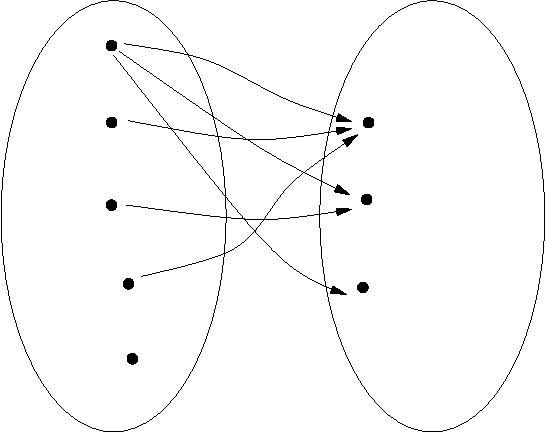
\includegraphics{figures/first_relation.pdf}%
\end{picture}%
\setlength{\unitlength}{3947sp}%
%
\begingroup\makeatletter\ifx\SetFigFont\undefined%
\gdef\SetFigFont#1#2#3#4#5{%
  \reset@font\fontsize{#1}{#2pt}%
  \fontfamily{#3}\fontseries{#4}\fontshape{#5}%
  \selectfont}%
\fi\endgroup%
\begin{picture}(4366,3466)(1193,-3819)
\put(1876,-811){\makebox(0,0)[lb]{\smash{{\SetFigFont{12}{14.4}{\familydefault}{\mddefault}{\updefault}{\color[rgb]{0,0,0}1}%
}}}}
\put(2026,-3286){\makebox(0,0)[lb]{\smash{{\SetFigFont{12}{14.4}{\familydefault}{\mddefault}{\updefault}{\color[rgb]{0,0,0}b}%
}}}}
\put(4276,-2011){\makebox(0,0)[lb]{\smash{{\SetFigFont{12}{14.4}{\familydefault}{\mddefault}{\updefault}{\color[rgb]{0,0,0}$\{1,3,5,7,\ldots\}$}%
}}}}
\put(4276,-1411){\makebox(0,0)[lb]{\smash{{\SetFigFont{12}{14.4}{\familydefault}{\mddefault}{\updefault}{\color[rgb]{0,0,0}$\{1,2,a\}$}%
}}}}
\put(4276,-2686){\makebox(0,0)[lb]{\smash{{\SetFigFont{12}{14.4}{\familydefault}{\mddefault}{\updefault}{\color[rgb]{0,0,0}$\{1\}$}%
}}}}
\put(2026,-2686){\makebox(0,0)[lb]{\smash{{\SetFigFont{12}{14.4}{\familydefault}{\mddefault}{\updefault}{\color[rgb]{0,0,0}a}%
}}}}
\put(1876,-1411){\makebox(0,0)[lb]{\smash{{\SetFigFont{12}{14.4}{\familydefault}{\mddefault}{\updefault}{\color[rgb]{0,0,0}2}%
}}}}
\put(1876,-2086){\makebox(0,0)[lb]{\smash{{\SetFigFont{12}{14.4}{\familydefault}{\mddefault}{\updefault}{\color[rgb]{0,0,0}3}%
}}}}
\end{picture}%

\caption[An example of a relation.]{The ``element of'' relation %
is an example of a relation that goes \emph{from} one set \emph{to} a %
different set.}
\label{fig:rel1} 
\end{figure}

A diagram such as we have given in Figure~\ref{fig:rel1} seems like a 
very natural thing.  Such pictures certainly give us an easy visual 
tool for thinking
about relations.  But we should point out certain hidden assumptions.
First, they'll only work if we are dealing with finite sets, or sets
like the odd numbers in our example (sets that are infinite but could
in principle be listed).  Second, by drawing the two sets separately,
it seems that we are assuming they are not only different, but 
\emph{disjoint}.  The sets not only need not be disjoint, but often
(most of the time!) we have relations that go from a set to itself
so the sets in a picture like this may be identical.  In Figure~\ref{fig:rel2}
we illustrate the divisibility relation on the set of all divisors of
6 --- this is an example in which the sets on either side of the relation
are the same.  Notice the linguistic distinction, we can talk about
either ``a relation from $A$ to $B$'' (when there are really two 
different sets) or ``a relation on $A$'' (when there is only one). 

\begin{figure}[!hbtp]
\begin{picture}(0,0)%
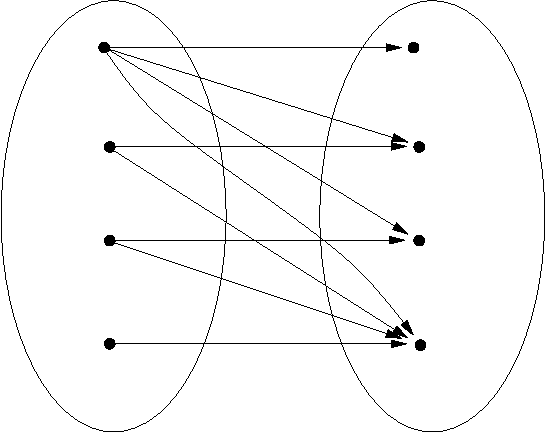
\includegraphics{./2nd_relation.pdf}%
\end{picture}%
\setlength{\unitlength}{3947sp}%
%
\begingroup\makeatletter\ifx\SetFigFont\undefined%
\gdef\SetFigFont#1#2#3#4#5{%
  \reset@font\fontsize{#1}{#2pt}%
  \fontfamily{#3}\fontseries{#4}\fontshape{#5}%
  \selectfont}%
\fi\endgroup%
\begin{picture}(4366,3466)(1193,-3819)
\put(1876,-3136){\makebox(0,0)[lb]{\smash{{\SetFigFont{12}{14.4}{\familydefault}{\mddefault}{\updefault}{\color[rgb]{0,0,0}6}%
}}}}
\put(1876,-2311){\makebox(0,0)[lb]{\smash{{\SetFigFont{12}{14.4}{\familydefault}{\mddefault}{\updefault}{\color[rgb]{0,0,0}3}%
}}}}
\put(1876,-1561){\makebox(0,0)[lb]{\smash{{\SetFigFont{12}{14.4}{\familydefault}{\mddefault}{\updefault}{\color[rgb]{0,0,0}2}%
}}}}
\put(1858,-763){\makebox(0,0)[lb]{\smash{{\SetFigFont{12}{14.4}{\familydefault}{\mddefault}{\updefault}{\color[rgb]{0,0,0}1}%
}}}}
\put(4678,-2302){\makebox(0,0)[lb]{\smash{{\SetFigFont{12}{14.4}{\familydefault}{\mddefault}{\updefault}{\color[rgb]{0,0,0}3}%
}}}}
\put(4678,-1548){\makebox(0,0)[lb]{\smash{{\SetFigFont{12}{14.4}{\familydefault}{\mddefault}{\updefault}{\color[rgb]{0,0,0}2}%
}}}}
\put(4637,-762){\makebox(0,0)[lb]{\smash{{\SetFigFont{12}{14.4}{\familydefault}{\mddefault}{\updefault}{\color[rgb]{0,0,0}1}%
}}}}
\put(4692,-3127){\makebox(0,0)[lb]{\smash{{\SetFigFont{12}{14.4}{\familydefault}{\mddefault}{\updefault}{\color[rgb]{0,0,0}6}%
}}}}
\end{picture}%

\caption[An example of the ``divides'' relation.]{The ``divides'' relation %
is an example of a relation that goes from a set to itself.  In this example %
we say that we have a relation \emph{on} the set of divisors of 6.}
\label{fig:rel2} 
\end{figure}
 
Purists will note that it is really inappropriate to represent the same set
in two different places in a Venn diagram.  The diagram in Figure~\ref{fig:rel2}
should really look like this:

\begin{center}
\begin{picture}(0,0)%
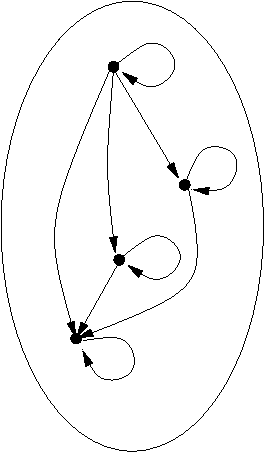
\includegraphics{figures/2nd_relation_v2.pdf}%
\end{picture}%
\setlength{\unitlength}{3947sp}%
%
\begingroup\makeatletter\ifx\SetFigFont\undefined%
\gdef\SetFigFont#1#2#3#4#5{%
  \reset@font\fontsize{#1}{#2pt}%
  \fontfamily{#3}\fontseries{#4}\fontshape{#5}%
  \selectfont}%
\fi\endgroup%
\begin{picture}(2116,3614)(1118,-3818)
\put(1876,-2311){\makebox(0,0)[lb]{\smash{{\SetFigFont{12}{14.4}{\familydefault}{\mddefault}{\updefault}{\color[rgb]{0,0,0}3}%
}}}}
\put(1858,-763){\makebox(0,0)[lb]{\smash{{\SetFigFont{12}{14.4}{\familydefault}{\mddefault}{\updefault}{\color[rgb]{0,0,0}1}%
}}}}
\put(1501,-2986){\makebox(0,0)[lb]{\smash{{\SetFigFont{12}{14.4}{\familydefault}{\mddefault}{\updefault}{\color[rgb]{0,0,0}6}%
}}}}
\put(2326,-1786){\makebox(0,0)[lb]{\smash{{\SetFigFont{12}{14.4}{\familydefault}{\mddefault}{\updefault}{\color[rgb]{0,0,0}2}%
}}}}
\end{picture}%

\end{center}

Indeed, this representation is definitely preferable, although it may be more crowded.  
A picture such as this is
known as the \index{directed graph}\emph{directed graph} (a.k.a. \index{digraph}\emph{digraph})
of the relation.

Recall that when we were discussing sets we said the best way to describe 
a set is simply to list all of its elements.  Well, what is the best
way to describe a relation?  In the same spirit, it would seem we should
explicitly list all the things that make the relation true.  But it takes
a \emph{pair} of things, one to go on the left side and one to go on the 
right, to make a relation true (or for that matter false!).  Also it should 
be evident that order is important in this context, for example $2<3$ is true
but $3<2$ isn't.  The identity of a relation is so intimately tied up with
the set of ordered pairs that make it true, that when dealing with abstract
relations we \emph{define them} as sets of ordered pairs.

Given two sets, $A$ and $B$, the \index{Cartesian product}
\emph{Cartesian product of $A$ and $B$} 
is the set of all ordered pairs $(a,b)$ where $a$ is in $A$ and $b$ is in $B$.
We denote the Cartesian product using the symbol $\times$.  

\[ A \times B = \{ (a,b) \suchthat a \in A \land b \in B \} \]

\noindent From here on out
in your mathematical career you'll need to take note of the context that
the symbol $\times$ appears in.  If it appears between numbers go ahead and
multiply, but if it appears between sets you're doing something different --
forming the Cartesian product.

The familiar $x$--$y$ plane, is often called the Cartesian plane.  This
is done for two reasons. \index{Descartes, Rene}Rene Descartes, the famous
mathematician and philosopher, was the first to consider coordinatizing
the plane and thus is responsible for our current understanding of the
relationship between geometry and algebra.  Rene Descartes' name is also
memorialized in the definition of the Cartesian product of sets, and the
plane is nothing more than the product $\Reals \times \Reals$.  Indeed,
the plane provided the very first example of the concept that was later
generalized to the Cartesian product of sets.

\begin{exer}
Suppose $A = \{1,2,3\}$ and $B = \{a,b,c\}$.  Is $(a,1)$ in the Cartesian
product $A \times B$?  List all elements of $A \times B$.
\end{exer} 

In the abstract, we can define a relation as \emph{any} subset of an
appropriate Cartesian product.  So an abstract relation $\relR$ from a set 
$A$ to a set $B$ is just some subset of $A \times B$.  Similarly, a
relation $\relR$ on a set $S$ is defined by a subset of $S \times S$.
This definition looks a little bit strange when we apply it to an
actual (concrete) relation that we already know about.  Consider the
relation ``less than.''   To describe ``less than'' as a subset of
a Cartesian product we must write

\[ < \; = \; \{ (x,y) \in \Reals \times \Reals \suchthat y-x \in \Reals^+ \}.\] 
\noindent This looks funny.

Also, if we have defined some relation $\relR \subseteq A \times B$, then in order
to say that a particular pair, $(a,b)$, of things make the relation true we
have to write 

\[ a\relR b. \]

\noindent This looks funny too.  

Despite the strange appearances, these 
examples do express the correct way to deal with relations.

Let's do a completely made-up example.  Suppose $A$ is the set
$\{a,e,i,o,u\}$ and $B$ is the set $\{r,s,t,l,n\}$ and we define 
a relation from $A$ to $B$ by

\[ \relR = \{ (a,s), (a,t), (a,n), (e,t), (e,l), (e,n), (i,s), (i,t), (o,r), (o,n), (u,s) \}. \]

Then, for example, because $(e,t) \in \relR$ we can write $e \relR t$.  We indicate the
negation of the concept that two elements are related by drawing a slash 
through the name of the relation, for example the notation $\neq$ is certainly
familiar to you, as is $\nless$ (although in this latter case we 
would normally write $\geq$ instead).  We can denote the fact that
$(a,l)$ is not a pair that makes the relation true by writing $a \nrelR l$.

We should mention another way of visualizing
relations.  When we are dealing with a relation on $\Reals$, the
relation is actually a subset of $\Reals \times \Reals$, that means 
we can view the relation as a subset of the $x$--$y$ plane.  In other 
words, we can graph it.  The graph of the ``$<$'' relation is
given in Figure~\ref{fig:lt_graph}.

\begin{figure}[!hbtp]
\begin{center}
\begin{picture}(0,0)%
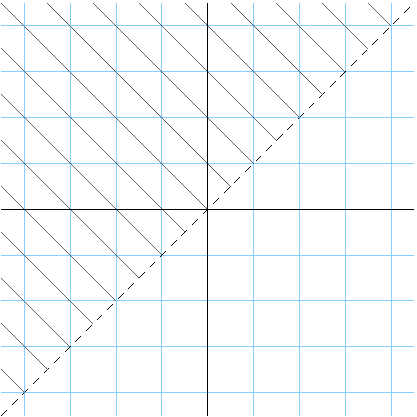
\includegraphics{figures/less_than_on_RxR.pdf}%
\end{picture}%
\setlength{\unitlength}{3947sp}%
%
\begingroup\makeatletter\ifx\SetFigFont\undefined%
\gdef\SetFigFont#1#2#3#4#5{%
  \reset@font\fontsize{#1}{#2pt}%
  \fontfamily{#3}\fontseries{#4}\fontshape{#5}%
  \selectfont}%
\fi\endgroup%
\begin{picture}(3324,3324)(1189,-3673)
\end{picture}%

\end{center}
\caption[The graph of the ``less than'' relation.]{The ``less than'' relation %
can be viewed as a subset of $\Reals \times \Reals$, i.e. it can be graphed.}
\label{fig:lt_graph} 
\end{figure}
  
A relation on any set that is a subset of $\Reals$ can likewise be
graphed.  The graph of the ``$\mid$'' relation is
given in Figure~\ref{fig:div_graph}.

\begin{figure}[!hbtp]
\begin{center}
\begin{picture}(0,0)%
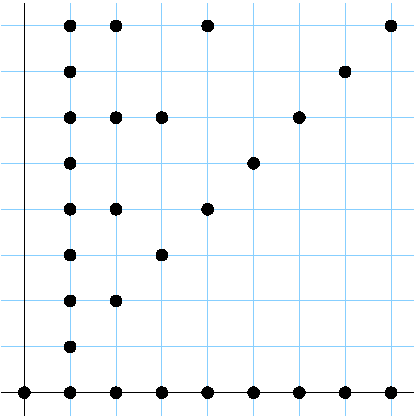
\includegraphics{figures/divides_on_NxN.pdf}%
\end{picture}%
\setlength{\unitlength}{3947sp}%
%
\begingroup\makeatletter\ifx\SetFigFont\undefined%
\gdef\SetFigFont#1#2#3#4#5{%
  \reset@font\fontsize{#1}{#2pt}%
  \fontfamily{#3}\fontseries{#4}\fontshape{#5}%
  \selectfont}%
\fi\endgroup%
\begin{picture}(3324,3324)(1189,-3673)
\end{picture}%

\end{center}
\caption[The graph of the divisibility relation.]{The divisibility relation %
can be graphed.  Only those points (as indicated) with integer coordinates %
are in the graph.}
\label{fig:div_graph} 
\end{figure}
 
Eventually, we will get around to defining functions as relations that
have a certain nice property.  For the moment, we'll just note that
some of the operations that you are used to using with functions
also apply with relations.  When one function ``undoes'' what another
function ``does'' we say the functions are inverses.  For example,
the function $f(x)=2x$ (i.e. doubling) and the function $g(x)=x/2$ (halving)
are inverse functions because, no matter what number we start with, if we
double it and then halve that result, we end up with the original number.
The \index{inverse, of a relation}inverse of a relation $\relR$ is written $\relR^{-1}$ and it consists of
the reversals of the pairs in $\relR$,

\[ \relR^{-1} = \{ (b,a) \suchthat (a,b) \in \relR \}. \]

This can also be expressed by writing

\[ b\relR^{-1}a \; \iff \; a\relR b. \]

The process of ``doing one function and then doing another'' is known
as \index{composition, of functions}functional composition.  For instance,
if $f(x) = 2x+1$ and $g(x) = \sqrt{x}$, then we can compose them (in two
different orders) to obtain either $f(g(x)) = 2\sqrt{x}+1$ or 
$g(f(x)) = \sqrt{2x+1}$.  When composing functions there is an ``intermediate
result'' that you get by applying the first function to your input, and then
you calculate the second function's value at the intermediate result.  
(For example, in calculating $g(f(4))$ we get the intermediate result
$f(4) = 9$ and then we go on to calculate $g(9) = 3$.)

The definition of the \index{composition, of relations}\emph{composite}
of two relations focuses very much on this idea
of the intermediate result.  Suppose $\relR$ is a relation from
$A$ to $B$ and $\relS$ is a relation from $B$ to $C$ then the composite
$\relS \circ \relR$ is given by

\[  \relS \circ \relR \; = \; \{ (a,c) \suchthat \exists b \in B, (a,b) \in \relR \, \land (b,c) \in \relS \}. \]

In this definition, $b$ is the ``intermediate result,'' if there is no such
$b$ that serves to connect $a$ to $c$ then $(a,c)$ won't be in the composite.
Also, notice that this is the composition $\relR$ first, then $\relS$, but
it is written as $\relS \circ \relR$  -- watch out for this!  The 
compositions of relations should be read from right to left.  This convention
makes sense when you consider functional composition, $f(g(x))$ means $g$ 
first, then $f$ so if we use the ``little circle'' notation for the
composition of relations we have $f \circ g (x) = f(g(x))$ which is nice
because the symbols $f$ and $g$ appear in the same order.  But beware! there
are atavists out there who write their compositions the other way around.

 
You should probably have a diagram like the following in mind while thinking
about the composition of relations.  Here, we have the set $A=\{1,2,3,4\}$,
the set $B$ is $\{a,b,c,d\}$ and $C=\{w,x,y,z\}$.  The relation
$\relR$ goes from $A$ to $B$ and consists of the following set of pairs,

\[ \relR \; = \; \{(1,a), (1,c), (2,d), (3,c), (3,d) \}. \]

And 

\[ \relS \; = \; \{(a,y), (b,w), (b,x), (b,z) \}. \]

\vfill

\begin{picture}(0,0)%
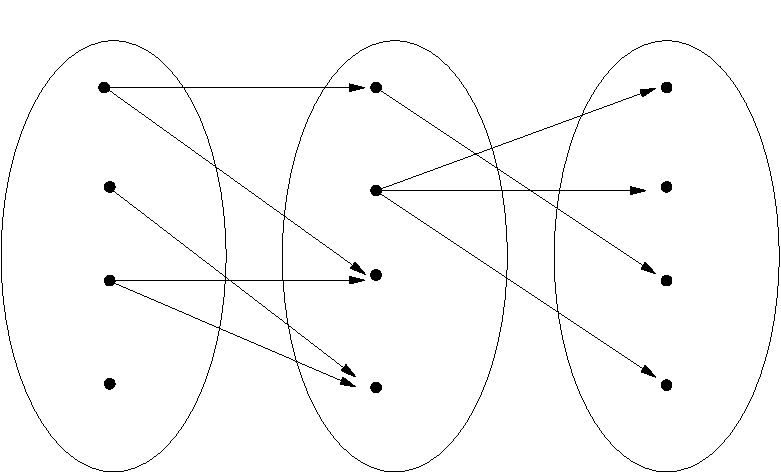
\includegraphics{./composite_relation.pdf}%
\end{picture}%
\setlength{\unitlength}{3947sp}%
%
\begingroup\makeatletter\ifx\SetFigFont\undefined%
\gdef\SetFigFont#1#2#3#4#5{%
  \reset@font\fontsize{#1}{#2pt}%
  \fontfamily{#3}\fontseries{#4}\fontshape{#5}%
  \selectfont}%
\fi\endgroup%
\begin{picture}(6241,3767)(1193,-3819)
\put(1876,-2311){\makebox(0,0)[lb]{\smash{{\SetFigFont{12}{14.4}{\familydefault}{\mddefault}{\updefault}{\color[rgb]{0,0,0}3}%
}}}}
\put(1876,-1561){\makebox(0,0)[lb]{\smash{{\SetFigFont{12}{14.4}{\familydefault}{\mddefault}{\updefault}{\color[rgb]{0,0,0}2}%
}}}}
\put(1858,-763){\makebox(0,0)[lb]{\smash{{\SetFigFont{12}{14.4}{\familydefault}{\mddefault}{\updefault}{\color[rgb]{0,0,0}1}%
}}}}
\put(1876,-3136){\makebox(0,0)[lb]{\smash{{\SetFigFont{12}{14.4}{\familydefault}{\mddefault}{\updefault}{\color[rgb]{0,0,0}4}%
}}}}
\put(3001,-286){\makebox(0,0)[lb]{\smash{{\SetFigFont{12}{14.4}{\familydefault}{\mddefault}{\updefault}{\color[rgb]{0,0,0}$\relR$}%
}}}}
\put(5701,-211){\makebox(0,0)[lb]{\smash{{\SetFigFont{12}{14.4}{\familydefault}{\mddefault}{\updefault}{\color[rgb]{0,0,0}$\relS$}%
}}}}
\put(4276,-3061){\makebox(0,0)[lb]{\smash{{\SetFigFont{12}{14.4}{\familydefault}{\mddefault}{\updefault}{\color[rgb]{0,0,0}d}%
}}}}
\put(4276,-661){\makebox(0,0)[lb]{\smash{{\SetFigFont{12}{14.4}{\familydefault}{\mddefault}{\updefault}{\color[rgb]{0,0,0}a}%
}}}}
\put(4276,-1486){\makebox(0,0)[lb]{\smash{{\SetFigFont{12}{14.4}{\familydefault}{\mddefault}{\updefault}{\color[rgb]{0,0,0}b}%
}}}}
\put(4276,-2161){\makebox(0,0)[lb]{\smash{{\SetFigFont{12}{14.4}{\familydefault}{\mddefault}{\updefault}{\color[rgb]{0,0,0}c}%
}}}}
\put(6676,-736){\makebox(0,0)[lb]{\smash{{\SetFigFont{12}{14.4}{\familydefault}{\mddefault}{\updefault}{\color[rgb]{0,0,0}w}%
}}}}
\put(6676,-1486){\makebox(0,0)[lb]{\smash{{\SetFigFont{12}{14.4}{\familydefault}{\mddefault}{\updefault}{\color[rgb]{0,0,0}x}%
}}}}
\put(6676,-2236){\makebox(0,0)[lb]{\smash{{\SetFigFont{12}{14.4}{\familydefault}{\mddefault}{\updefault}{\color[rgb]{0,0,0}y}%
}}}}
\put(6676,-3061){\makebox(0,0)[lb]{\smash{{\SetFigFont{12}{14.4}{\familydefault}{\mddefault}{\updefault}{\color[rgb]{0,0,0}z}%
}}}}
\end{picture}%


\begin{exer}
Notice that the composition $\relR \circ \relS$ is impossible (or, more
properly, it is empty).  Why?

What is the (only) pair in the composition $\relS \circ \relR$ ?
\end{exer}

\newpage

\noindent{\large \bf Exercises --- \thesection\ }

\begin{enumerate}
\item The \index{lexicographic order}\emph{lexicographic order}, 
$<_{\mbox{lex}}$, is a relation on the
set of all words, where $x <_{\mbox{lex}} y$ means that $x$ would come before
$y$ in the dictionary.  Consider just the three letter words like ``iff'',
``fig'', ``the'', et cetera.  Come up with a usable definition for
$x_1x_2x_3  <_{\mbox{lex}} y_1y_2y_3$.

\item What is the graph of ``$=$'' in $\Reals \times \Reals$?

\item The \index{inverse relation} \emph{inverse} of a relation $\relR$
is denoted $\relR^{-1}$.  It contains exactly the same ordered pairs
as $\relR$ but with the order switched.  (So technically, they aren't
\emph{exactly} the same ordered pairs \ldots)

\[ \relR^{-1} = \{ (b,a) \suchthat (a,b) \in \relR \} \]

\noindent Define a relation $\relS$ on $\Reals \times \Reals$ by
$\relS = \{ (x,y) \suchthat y = \sin x \}$.  What is $\relS^{-1}$?
Draw a single graph containing $\relS$ and $\relS^{-1}$.

\item The ``socks and shoes'' rule is a very silly little mnemonic
for remembering how to invert a composition.  If we think of undoing
the process of putting on our socks and shoes (that's socks first, then
shoes) we have to first remove our shoes, \emph{then} take off our socks.

The socks and shoes rule is valid for relations as well.

Prove that $(\relS \circ \relR)^{-1} = \relR^{-1} \circ \relS^{-1}$.

\end{enumerate} 

%% Emacs customization
%% 
%% Local Variables: ***
%% TeX-master: "GIAM-hw.tex" ***
%% comment-column:0 ***
%% comment-start: "%% "  ***
%% comment-end:"***" ***
%% End: ***



\newpage

\section{Properties of relations}
\label{sec:rel_props}

There are two special classes of relations that we will study
in the next two sections, equivalence relations and ordering relations.
The prototype for an equivalence relation is the ordinary notion
of numerical equality, $=$.  The prototypical ordering relation
is $\leq$.  Each of these has certain salient properties that are the
root causes of their importance.  In this section we will study a 
compendium of properties that a relation may or may not have.  

A relation that has three of the properties we'll discuss:

\begin{enumerate}
\item \index{reflexivity} reflexivity 
\item \index{symmetry}symmetry 
\item \index{transitivity}transitivity
\end{enumerate}

\noindent is said to be an equivalence relation; it will in some ways resemble
$=$.

A relation that has another set of three properties:

\begin{enumerate}
\item \index{reflexivity}reflexivity 
\item \index{anti-symmetry}anti-symmetry 
\item \index{transitivity}transitivity
\end{enumerate}

\noindent is called an ordering relation; it will resemble $\leq$.

Additionally, there is a property known as irreflexivity that many
relations have.

There are a total of 5 properties that we have named, and we will discuss
them all more thoroughly.  But first, we'll state the formal definitions.
Take note that these properties are all stated for a relation that goes
from a set to itself, indeed, most of them wouldn't even make sense if
we tried to define them for a relation from a set to a different set.

\clearpage

\begin{table}[hbt] 
\begin{center}
\begin{tabular}{|c|} \hline
\begin{minipage}{.95\textwidth} \centerline{\rule{0pt}{15pt} A relation $\relR$ on a set $S$ is {\bf reflexive} iff} 
\rule{0pt}{15pt} \centerline{ $\displaystyle \forall a \in S, \quad a \relR a $} 
\rule[-6pt]{0pt}{21pt} ``Everything is related to itself.''
\end{minipage} \\ \hline
\begin{minipage}{.95\textwidth} \centerline{\rule{0pt}{15pt}A relation $\relR$ on a set $S$ is {\bf irreflexive} iff}
\rule{0pt}{15pt} \centerline{ $\displaystyle \forall a \in S, \quad a \nrelR a $ }
\rule[-6pt]{0pt}{21pt} ``Nothing is related to itself.''
\end{minipage} \\ \hline
\begin{minipage}{.95\textwidth} \centerline{\rule{0pt}{15pt}A relation $\relR$ on a set $S$ is {\bf symmetric} iff}
\rule{0pt}{15pt} \centerline{ $\displaystyle \forall a,b \in S, \quad a \relR b \; \implies \; b \relR a $ }
\rule[-6pt]{0pt}{21pt} ``No one-way streets.'' 
\end{minipage} \\ \hline
\begin{minipage}{.95\textwidth} \centerline{\rule{0pt}{15pt}A relation $\relR$ on a set $S$ is {\bf anti-symmetric} iff}
\rule{0pt}{15pt} \centerline{ $\displaystyle \forall a,b \in S, \quad a \relR b \; \land b \relR a \quad \implies \quad a=b $}
\rule[-6pt]{0pt}{21pt} ``Only one-way streets.''
\end{minipage} \\ \hline
\begin{minipage}{.95\textwidth} \centerline{\rule{0pt}{15pt}A relation $\relR$ on a set $S$ is {\bf transitive} iff}
\rule{0pt}{15pt} \centerline{ $\displaystyle \forall a,b,c \in S, \quad a \relR b \; \land \; b \relR c \quad \implies \quad a \relR c$ }
\rule[-6pt]{0pt}{21pt} ``Whenever there's a roundabout route, there's a direct route.''
\end{minipage} \\ \hline
\end{tabular} 
\end{center} 
\caption[Properties of relations.]{Properties that relations may (or may not) have.}
\index{Properties of relations}
\label{tab:rel_props}
\end{table}


The digraph of a relation that is reflexive will have little loops at every vertex.
The digraph of a relation that is irreflexive will contain no loops at all.
Hopefully it is clear that these concepts represent extreme opposite possibilities --
they are \emph{not} however negations of one another.

\begin{exer}
Find the logical denial of the property that says a relation is reflexive

\[ {\lnot}(\forall a \in S, \quad a \relR a). \]

How does this differ from the defining property for ``irreflexive''?
\end{exer}

If a relation $\relR$ is defined on some subset $S$ of the reals, then it can be graphed
in the Euclidean plane.  Reflexivity for $\relR$ can be interpreted in terms of the line
$L$ defined by the equation $y=x$.  Every point in $(S \times S) \cap L$
must be in $\relR$.  A similar statement can be made concerning the irreflexive property.
If a relation $\relR$ is irreflexive its graph completely avoids the line $y=x$.

Note that the reflexive and irreflexive properties are defined with a single quantified
variable.  Symmetry and anti-symmetry require two universally quantified variables for
their definitions.

\begin{quote}
A relation $\relR$ on a set $S$ is {\bf symmetric} iff
\[ \forall a,b \in S, \quad a \relR b \; \implies \; b \relR a. \] 
\end{quote}

\noindent This can be interpreted in terms of digraphs as follows:  If a connection
from $a$ to $b$ exists in the digraph of $\relR$, then there must also be a connection
from $b$ to $a$.   In Table~\ref{tab:rel_props} this is interpreted as ``no one-way streets''
and while that's not quite what it says, that \emph{is} the effect of this definition.
Since \emph{if} a connection exists in one direction, there must also be a connection 
in the other direction, it follows that we will never see a one-way connection.

Because most of the properties we are studying are defined using conditional statements
it is often the case that a relation has a property for vacuous reasons.  When the ``if'' part
doesn't happen, there's no need for its corresponding ``then'' part to happen either -- the 
conditional is still true.  In the context of our discussion on the symmetry property of
a relation this means that the following digraph \emph{is} the digraph of a symmetric
relation (although it is neither reflexive nor irreflexive).

\begin{center}
\begin{picture}(0,0)%
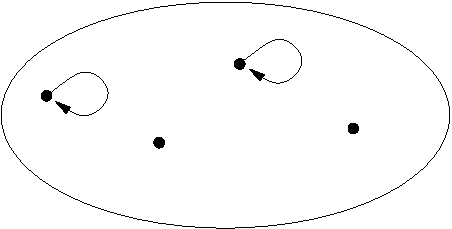
\includegraphics{./vacuously_symmetric.pdf}%
\end{picture}%
\setlength{\unitlength}{3947sp}%
%
\begingroup\makeatletter\ifx\SetFigFont\undefined%
\gdef\SetFigFont#1#2#3#4#5{%
  \reset@font\fontsize{#1}{#2pt}%
  \fontfamily{#3}\fontseries{#4}\fontshape{#5}%
  \selectfont}%
\fi\endgroup%
\begin{picture}(3606,1822)(1653,-1801)
\put(1824,-774){\makebox(0,0)[lb]{\smash{{\SetFigFont{12}{14.4}{\familydefault}{\mddefault}{\updefault}{\color[rgb]{0,0,0}a}%
}}}}
\put(2701,-1186){\makebox(0,0)[lb]{\smash{{\SetFigFont{12}{14.4}{\familydefault}{\mddefault}{\updefault}{\color[rgb]{0,0,0}b}%
}}}}
\put(3376,-511){\makebox(0,0)[lb]{\smash{{\SetFigFont{12}{14.4}{\familydefault}{\mddefault}{\updefault}{\color[rgb]{0,0,0}c}%
}}}}
\put(4276,-1036){\makebox(0,0)[lb]{\smash{{\SetFigFont{12}{14.4}{\familydefault}{\mddefault}{\updefault}{\color[rgb]{0,0,0}d}%
}}}}
\end{picture}%

\end{center}

Anti-symmetry is described as meaning ``only one-way streets'' but the definition is given
as:

\begin{quote}
A relation $\relR$ on a set $S$ is {\bf anti-symmetric} iff \newline
\centerline{ $\displaystyle \forall a,b \in S, \quad a \relR b \; \land b \relR a \quad \implies \quad a=b$.}
\end{quote}

It may be hard at first to understand why the definition we use for anti-symmetry is the one above.
If one wanted to insure that there were never two-way connections between elements of the set it
might seem easier to define anti-symmetry as follows:

\begin{quote}
(Alternate definition) A relation $\relR$ on a set $S$ is {\bf anti-symmetric} iff \newline
\centerline{ $\displaystyle \forall a,b \in S, \quad a \relR b \; \implies \; b \nrelR a$.}
\end{quote}

This definition may seem more straight-forward, but it turns out the original definition is
easier to use in proofs.  We need to convince ourselves that the (first) definition really
accomplishes what we want.  Namely, if a relation $\relR$ satisfies the property that
$\displaystyle \forall a,b \in S, \quad a \relR b \; \land \; b \relR a \quad \implies \quad a=b$,
then there will not actually be any pair of elements that are related in both orders.  One
way to think about it is this: suppose that $a$ and $b$ are distinct elements of $S$ and
that both $a \relR b$ and $b \relR a$ are true.  The property now guarantees that $a=b$
which contradicts the notion that $a$ and $b$ are distinct.  This is a miniature proof
by contradiction; if you assume there \emph{are} a pair of distinct elements that are
related in both orders you get a contradiction, so there \emph{aren't}!

A funny thing about the anti-symmetry property is this:  When it is true of a relation it 
is \emph{always} vacuously true!  The property is engineered in such a way that when it is
true, it forces that the statement in its antecedent never really happens.

Transitivity is an extremely useful property as witnessed by the fact that both equivalence
relations and ordering relations must have this property.  When speaking of the transitive
property of equality we say ``Two things that are equal to a third, are equal to each other.''
When dealing with ordering we may encounter statements like the following.  
``Since `Aardvark' precedes `Bulwark'  %
in the dictionary, and since `Bulwark' precedes `Catastrophe', it is plainly true that `Aardvark'  %
comes before `Catastrophe' in the dictionary.''

Again, the definition of transitivity involves a conditional.  Also, transitivity may be viewed 
as the most complicated of the properties we've been studying; it takes three universally 
quantified variables to state the property.

\begin{quote}
A relation $\relR$ on a set $S$ is {\bf transitive} iff \newline
\centerline{ $\displaystyle \forall a,b,c \in S, \quad a \relR b \; \land \; b \relR c \quad \implies \quad a \relR c$ }
\end{quote}

We paraphrased transitivity as  ``Whenever there's a roundabout route, there's a direct route.''
In particular, what the definition says is that \emph{if} there's a connection from $a$ to $b$ and from
$b$ to $c$ (the roundabout route from $a$ to $c$) then there must be a connection from $a$ to $c$ (the direct
route).  

You'll really need to watch out for relations that are transitive for vacuous reasons.  So long as one
never has three elements $a$, $b$ and $c$ with $a \relR b$ and $b \relR c$ the statement that defines
transitivity is automatically true.

A very useful way of thinking about these various properties that relations may have is in terms of 
what \emph{doesn't} happen when a relation has them.  Before we proceed, it is important that 
you do the following

\begin{exer}
Find logical negations for the formal properties defining each of the five
properties.
\end{exer}

\newpage

If a relation $\relR$ is reflexive we will never see a node that doesn't have a loop.

\begin{center}
\begin{picture}(0,0)%
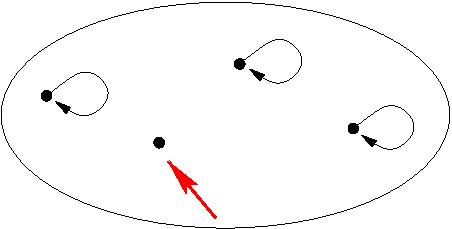
\includegraphics{figures/not_reflexive.pdf}%
\end{picture}%
\setlength{\unitlength}{3947sp}%
%
\begingroup\makeatletter\ifx\SetFigFont\undefined%
\gdef\SetFigFont#1#2#3#4#5{%
  \reset@font\fontsize{#1}{#2pt}%
  \fontfamily{#3}\fontseries{#4}\fontshape{#5}%
  \selectfont}%
\fi\endgroup%
\begin{picture}(3606,1822)(1653,-1801)
\put(1824,-774){\makebox(0,0)[lb]{\smash{{\SetFigFont{12}{14.4}{\familydefault}{\mddefault}{\updefault}{\color[rgb]{0,0,0}a}%
}}}}
\put(2701,-1186){\makebox(0,0)[lb]{\smash{{\SetFigFont{12}{14.4}{\familydefault}{\mddefault}{\updefault}{\color[rgb]{0,0,0}b}%
}}}}
\put(3376,-511){\makebox(0,0)[lb]{\smash{{\SetFigFont{12}{14.4}{\familydefault}{\mddefault}{\updefault}{\color[rgb]{0,0,0}c}%
}}}}
\put(4276,-1036){\makebox(0,0)[lb]{\smash{{\SetFigFont{12}{14.4}{\familydefault}{\mddefault}{\updefault}{\color[rgb]{0,0,0}d}%
}}}}
\end{picture}%

\end{center}

\vfill

If a relation $\relR$ is irreflexive we will never see a node that \emph{does} have a loop!

\begin{center}
\begin{picture}(0,0)%
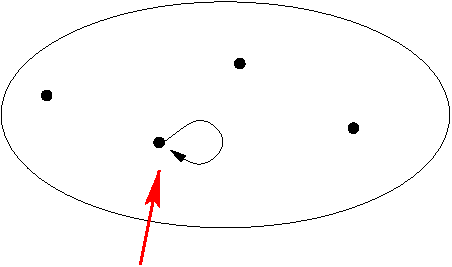
\includegraphics{./not_irreflexive.pdf}%
\end{picture}%
\setlength{\unitlength}{3947sp}%
%
\begingroup\makeatletter\ifx\SetFigFont\undefined%
\gdef\SetFigFont#1#2#3#4#5{%
  \reset@font\fontsize{#1}{#2pt}%
  \fontfamily{#3}\fontseries{#4}\fontshape{#5}%
  \selectfont}%
\fi\endgroup%
\begin{picture}(3606,2129)(1653,-2108)
\put(1824,-774){\makebox(0,0)[lb]{\smash{{\SetFigFont{12}{14.4}{\familydefault}{\mddefault}{\updefault}{\color[rgb]{0,0,0}a}%
}}}}
\put(2701,-1186){\makebox(0,0)[lb]{\smash{{\SetFigFont{12}{14.4}{\familydefault}{\mddefault}{\updefault}{\color[rgb]{0,0,0}b}%
}}}}
\put(3376,-511){\makebox(0,0)[lb]{\smash{{\SetFigFont{12}{14.4}{\familydefault}{\mddefault}{\updefault}{\color[rgb]{0,0,0}c}%
}}}}
\put(4276,-1036){\makebox(0,0)[lb]{\smash{{\SetFigFont{12}{14.4}{\familydefault}{\mddefault}{\updefault}{\color[rgb]{0,0,0}d}%
}}}}
\end{picture}%

\end{center}

\vfill

If a relation $\relR$ is symmetric we will never see a pair of nodes that are connected in one
direction only.

\begin{center}
\begin{picture}(0,0)%
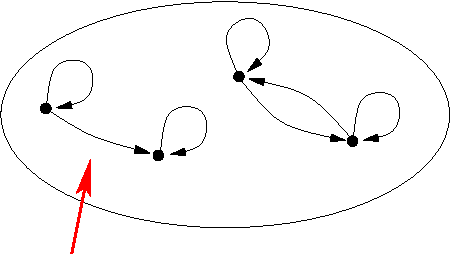
\includegraphics{figures/not_symmetric.pdf}%
\end{picture}%
\setlength{\unitlength}{3947sp}%
%
\begingroup\makeatletter\ifx\SetFigFont\undefined%
\gdef\SetFigFont#1#2#3#4#5{%
  \reset@font\fontsize{#1}{#2pt}%
  \fontfamily{#3}\fontseries{#4}\fontshape{#5}%
  \selectfont}%
\fi\endgroup%
\begin{picture}(3606,2041)(1659,-1916)
\put(1824,-774){\makebox(0,0)[lb]{\smash{{\SetFigFont{12}{14.4}{\familydefault}{\mddefault}{\updefault}{\color[rgb]{0,0,0}a}%
}}}}
\put(3376,-511){\makebox(0,0)[lb]{\smash{{\SetFigFont{12}{14.4}{\familydefault}{\mddefault}{\updefault}{\color[rgb]{0,0,0}c}%
}}}}
\put(2981,-1333){\makebox(0,0)[lb]{\smash{{\SetFigFont{12}{14.4}{\familydefault}{\mddefault}{\updefault}{\color[rgb]{0,0,0}b}%
}}}}
\put(4430,-1243){\makebox(0,0)[lb]{\smash{{\SetFigFont{12}{14.4}{\familydefault}{\mddefault}{\updefault}{\color[rgb]{0,0,0}d}%
}}}}
\end{picture}%

\end{center}

\vfill

\newpage

If a relation $\relR$ is anti-symmetric we will never see a pair of nodes that are connected in both
directions.

\begin{center}
\begin{picture}(0,0)%
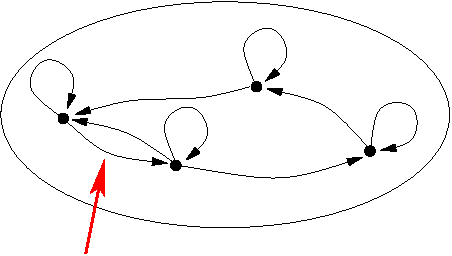
\includegraphics{figures/not_anti-symmetric.pdf}%
\end{picture}%
\setlength{\unitlength}{3947sp}%
%
\begingroup\makeatletter\ifx\SetFigFont\undefined%
\gdef\SetFigFont#1#2#3#4#5{%
  \reset@font\fontsize{#1}{#2pt}%
  \fontfamily{#3}\fontseries{#4}\fontshape{#5}%
  \selectfont}%
\fi\endgroup%
\begin{picture}(3606,2041)(1519,-1836)
\put(1824,-774){\makebox(0,0)[lb]{\smash{{\SetFigFont{12}{14.4}{\familydefault}{\mddefault}{\updefault}{\color[rgb]{0,0,0}a}%
}}}}
\put(2981,-1333){\makebox(0,0)[lb]{\smash{{\SetFigFont{12}{14.4}{\familydefault}{\mddefault}{\updefault}{\color[rgb]{0,0,0}b}%
}}}}
\put(3369,-444){\makebox(0,0)[lb]{\smash{{\SetFigFont{12}{14.4}{\familydefault}{\mddefault}{\updefault}{\color[rgb]{0,0,0}c}%
}}}}
\put(4470,-1196){\makebox(0,0)[lb]{\smash{{\SetFigFont{12}{14.4}{\familydefault}{\mddefault}{\updefault}{\color[rgb]{0,0,0}d}%
}}}}
\end{picture}%

\end{center}

\vfill

If a relation $\relR$ is transitive the thing we will never see is a bit harder to describe.
There will never be a pair of arrows meeting head to tail \emph{without} there also being an
arrow going from the tail of the first to the head of the second. 

\begin{center}
\begin{picture}(0,0)%
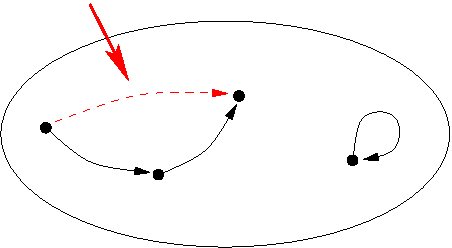
\includegraphics{figures/not_transitive.pdf}%
\end{picture}%
\setlength{\unitlength}{3947sp}%
%
\begingroup\makeatletter\ifx\SetFigFont\undefined%
\gdef\SetFigFont#1#2#3#4#5{%
  \reset@font\fontsize{#1}{#2pt}%
  \fontfamily{#3}\fontseries{#4}\fontshape{#5}%
  \selectfont}%
\fi\endgroup%
\begin{picture}(3606,1970)(1659,-1697)
\put(1824,-774){\makebox(0,0)[lb]{\smash{{\SetFigFont{12}{14.4}{\familydefault}{\mddefault}{\updefault}{\color[rgb]{0,0,0}a}%
}}}}
\put(2981,-1333){\makebox(0,0)[lb]{\smash{{\SetFigFont{12}{14.4}{\familydefault}{\mddefault}{\updefault}{\color[rgb]{0,0,0}b}%
}}}}
\put(4430,-1243){\makebox(0,0)[lb]{\smash{{\SetFigFont{12}{14.4}{\familydefault}{\mddefault}{\updefault}{\color[rgb]{0,0,0}d}%
}}}}
\put(3543,-391){\makebox(0,0)[lb]{\smash{{\SetFigFont{12}{14.4}{\familydefault}{\mddefault}{\updefault}{\color[rgb]{0,0,0}c}%
}}}}
\end{picture}%

\end{center}

\vfill

\newpage

\noindent{\large \bf Exercises --- \thesection\ }

\begin{enumerate}
\item Consider the relation $\relS$ defined by 
$ \relS = \{ (x,y) \suchthat \; x \, \mbox{is smarter than} \, y \}$.
Is $\relS$ symmetric or anti-symmetric?  Explain.

\wbvfill

\item Consider the relation $\relA$ defined by 
$ \relA = \{ (x,y) \suchthat \; x \, \mbox{has the same astrological sign as} \, y \}$.
Is $\relA$ symmetric or anti-symmetric?  Explain.

\wbvfill

\item Explain why both of the relations just described (in problems 1 and 2)
have the transitive property.

\wbvfill

\item For each of the five properties, name a relation that has it
and a relation that doesn't.

\wbvfill

\rule{0pt}{0pt}

\wbvfill

\workbookpagebreak

\item Show by counterexample that ``$\divides$'' (divisibility) is not symmetric as a relation on $\Integers$.

 \wbvfill
 
 \item Prove that ``$\divides$'' is an ordering relation (you must verify that it is reflexive, anti-symmetric and transitive).

 \wbvfill

\rule{0pt}{0pt}

\end{enumerate} 

%% Emacs customization
%% 
%% Local Variables: ***
%% TeX-master: "GIAM-hw.tex" ***
%% comment-column:0 ***
%% comment-start: "%% "  ***
%% comment-end:"***" ***
%% End: ***


\newpage

\section{Equivalence relations}
\label{sec:eq_rel}

The main idea of an equivalence relation is that it is something like
equality, but not quite.  Usually there is some property that 
we can name, so that equivalent things share that property.  For 
example Albert Einstein and Adolf Eichmann were two entirely
different human beings, if you consider all the different criteria
that one can use to distinguish human beings there is little they
have in common.  But, if the only thing one was interested in was
a person's initials, one would have to say that Einstein and Eichmann
were equivalent.  Future examples of equivalence relations will
be less frivolous\ldots  But first, the formal definition:

\begin{defi} A relation $\relR$ on a set $S$ is an \index{equivalence relation}\emph{equivalence relation}
iff $\relR$ is reflexive, symmetric and transitive.
\end{defi}

Probably the most important equivalence relation we've seen to date
is ``congruence mod $m$'' which we will denote using the symbol $\equiv_m$.
This relation may even be more interesting than
actual equality!   The reason for this seemingly odd statement is that
``congruence mod $m$'' gives us non-trivial \index{equivalence class} equivalence classes.  Equivalence
classes are one of the most potent ideas in modern mathematics and it's essential
that you understand them, so we'll start with an example.  Consider congruence
mod $5$.  What other numbers is (say) 11 equivalent to?  There are many!  Any 
number that leaves the same remainder as 11 when we divide it by 5.  This collection
is called the equivalence class of 11 and is usually denoted using an overline --- 
$\overline{11}$, another notation that is often seen for the set of things equivalent 
to 11 is $11/\equiv_5$. 

\[ \overline{11} = \{ \ldots, -9, -4, 1, 6, 11, 16, \ldots \} \]

It's easy to see that we will get the exact same set if we choose any other element
of the equivalence class (in place of 11), which leads us to an infinite list of set
equalities,

\[   \overline{1} = \overline{6} = \overline{11} = \ldots \]

\noindent And similarly, 

\[   \overline{2} = \overline{7} = \overline{12} = \ldots \]

\noindent In fact, there are really just 5 different sets that form the
equivalence classes mod 5:  $\overline{0}$, $\overline{1}$, $\overline{2}$, $\overline{3}$, 
and $\overline{4}$.  (Note: we have followed the usual convention of using the smallest
 possible non-negative integers as the representatives for our equivalence classes.)

What we've been discussing here is one of the first examples of a \index{quotient structure}
\emph{quotient structure}.
We start with the integers and ``mod out'' by an equivalence relation.  In doing so, we
``move to the quotient'' which means (in this instance) that we go from $\Integers$ to a much simpler set
having only five elements: $\{ \overline{0}, \overline{1}, \overline{2}, \overline{3}, 
\overline{4} \}$.  In moving to the quotient we will generally lose a lot of information, 
but greatly highlight some particular feature -- in this example, properties related to 
divisibility by 5.
 
Given some equivalence relation $\relR$ defined on a set $S$ the set of equivalence classes
of $S$ under $\relR$ is denoted $S/\relR$ (which is read ``$S$ mod $\relR$'').  This use of the
slash -- normally reserved for division -- shouldn't cause any confusion since those aren't 
numbers on either side of the slash but rather a set and a relation.  This
notation may also clarify why some people denote the equivalence classes above
by $0/\equiv_5$, $1/\equiv_5$, $2/\equiv_5$, $3/\equiv_5$ and  $4/\equiv_5$.
 
The set of equivalence
classes forms a \index{partition} \emph{partition} of the set $S$.

\begin{defi} A \emph{partition} $P$ of a set $S$ is a set of sets such that

\[ S = \bigcup_{X \in P} X \qquad \mbox{and} \qquad %
\forall X, Y \in P, \; X \neq Y \, \implies \, X \cap Y = \emptyset. \]

\end{defi}
 
In words, if you take the union of all the pieces of the partition you'll get the
set $S$, and any pair of sets from the partition that aren't identical are disjoint.  
Partitions are an inherently useful way of looking at things, although in the real world
there are often problems (sets we thought were disjoint turn out to have elements in common,
or we discover something that doesn't fit into any of the pieces of our partition), in
mathematics we usually find that partitions do just what we would want them to do.  
Partitions divide some set up into a number of convenient pieces in such a way that we're
guaranteed that every element of the set is in one of the pieces and also so that none of
the pieces overlap.  Partitions are a useful way of dissecting sets, and equivalence relations
(via their equivalence classes) give us an easy way of creating partitions --
usually with some additional structure to boot!  The 
properties that make a relation an equivalence relation (reflexivity, symmetry and 
transitivity) are designed to ensure that equivalence classes exist and do provide us
with the desired partition.  For the beginning proof writer this all may seem very complicated,
but take heart!  Most of the work has already been done for you by those who created
the general theory of equivalence relations and quotient structures.  All you have
to do (usually) is prove that a given relation is an equivalence relation by verifying
that it is indeed reflexive, symmetric and transitive.  Let's have a look at another
example.

In Number Theory, the \index{square-free part, of an integer} square-free part of an integer is what remains after we divide-out
the largest perfect square that divides it.  (This is also known as the 
\index{radical, of an integer}\emph{radical} of an integer.)  
The following table gives the
square-free part, $sf(n)$, for the first several values of $n$.

\begin{center}
\begin{tabular}{c|cccccccccccccccccccc}
$n$ & 1 & 2 & 3 & 4 & 5 & 6 & 7 & 8 & 9 & 10 & 11 & 12 & 13 & 14 & 15 & 16 & 17 & 18 & 19 & 20 \\ \hline
$sf(n)$ & 1 & 2 & 3 & 1& 5 & 6 & 7  & 2  & 1 & 10 & 11  & 3 & 13 & 14 & 15 & 1 & 17 & 2  & 19 & 5 \\
\end{tabular}
\end{center}  

It's easy to compute the square-free part of an integer if you know its prime factorization
-- just reduce all the exponents mod 2.  For example\footnote{This is the size of largest 
sporadic finite simple group, known as ``the Monster.''}

\begin{gather*} 
808017424794512875886459904961710757005754368000000000 \\ 
 = 2^{46}\cdot 3^{20}\cdot 5^9\cdot7^6\cdot 11^2\cdot 13^3\cdot 17
\cdot 19\cdot 23\cdot 29\cdot 31\cdot 41\cdot 47\cdot 59\cdot 71
\end{gather*}

\noindent the square-free part of this number is 

\begin{gather*} 
5\cdot 13\cdot 17\cdot 19\cdot 23\cdot 29\cdot 31\cdot 41\cdot 47\cdot 59\cdot 71\\
 = 3504253225343845
\end{gather*}

\noindent which, while it is still quite a large number, is certainly a good
bit smaller than the original!

We will define an equivalence relation $\relS$ on the set of natural numbers
by using the square-free part:  

\[ \forall x, y \in \Naturals, \; x \relS y \; \iff sf(x) = sf(y) \]

In other words, two natural numbers will be $\relS$-related if they have the
same square-free parts.

\begin{exer}
What is $1/\relS$?
\end{exer}

Before we proceed to the proof that $\relS$ is an equivalence relation we'd like 
you to be cognizant of a bigger picture as you read.  Each of the three parts of
the proof will have a similar structure.  We will show that $\relS$ has one of the 
three properties by using the fact that $=$ has that property.  In more advanced
work this entire proof could be omitted or replaced by the phrase ``$\relS$ inherits
reflexivity, symmetry and transitivity from equality, and is therefore an equivalence
relation.''  (Nice trick isn't it?  But before you're allowed to use it you have
to show that you can do it the hard way \ldots)

\begin{thm} 
The relation $\relS$ defined by
\[ \forall x, y \in \Naturals, \; x \relS y \; \iff sf(x) = sf(y) \]
\noindent is an equivalence relation on $\Naturals$.
\end{thm}

\begin{proof}
We must show that $\relS$ is reflexive, symmetric and transitive.

{\bf reflexive} --- (Here we must show that $\forall x \in \Naturals, \; x \relS x$.)
Let $x$ be an arbitrary natural number.  Since $sf(x) = sf(x)$ (this is the reflexive 
property of $=$) it follows from the definition of $\relS$ that $x \relS x$.

{\bf symmetric} --- (Here we must show that  $\forall x,y \in \Naturals, \; x \relS y \, 
\implies \, y \relS x$.)
Let $x$ and $y$ be arbitrary natural numbers, and further suppose that $x \relS y$. 
Since $x \relS y$, it follows from the definition of $\relS$ that $sf(x) = sf(y)$,
obviously then $sf(y) = sf(x)$ (this is the symmetric property of $=$) and so 
$y \relS x$.

{\bf transitive} --- (Here we must show that  $\forall x,y,z \in \Naturals, \; x \relS y \,
\land \, y \relS z \; \implies \; x \relS z$.)
Let $x$, $y$ and $z$ be arbitrary natural numbers, and further suppose that both 
$x \relS y$ and $y \relS z$.  From the definition of $\relS$ we deduce that 
$sf(x) = sf(y)$ and $sf(y) = sf(z)$.  Clearly, $sf(x) = sf(z)$ (this deduction comes
from the transitive property of $=$), so $x \relS z$.

\end{proof}
 
We'll end this section with an example of an equivalence relation that
doesn't ``inherit'' the three properties from equality.  

A \index{graph} \emph{graph} is a mathematical structure consisting of
two sets, a set $V$ of points (a.k.a. vertices) and a set\footnote{Technically, $E$ is a so-called
multiset in many instances -- there may be several edges that connect the same pair of vertices.} $E$ of edges.
The elements of $E$ may be either ordered or unordered pairs from $V$. 
If $E$ consists of ordered pairs we have a \index{digraph} 
\emph{directed graph} or \emph{digraph} -- the diagrams we have been using to visualize
relations!  If $E$ consists of unordered 
pairs then we are dealing with an \emph{undirected graph}.  Since the
undirected case is actually the more usual, if the word ``graph'' appears without
a modifier it is assumed that we are talking about an undirected graph.

The previous paragraph gives a relatively precise definition of a graph
in terms of sets, however the real way to think of graphs is in terms
of diagrams where a set of dots are connected by paths.  (The paths will, 
of course, need to
have arrows on them in digraphs.)  Below are a few examples of the 
diagrams that are used to represent graphs.

\begin{center}
\begin{picture}(0,0)%
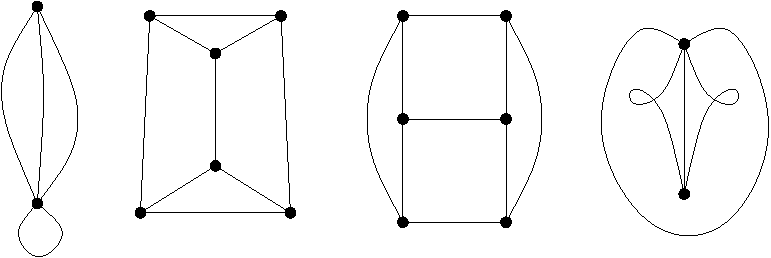
\includegraphics{figures/graph_examples.pdf}%
\end{picture}%
\setlength{\unitlength}{3947sp}%
%
\begingroup\makeatletter\ifx\SetFigFont\undefined%
\gdef\SetFigFont#1#2#3#4#5{%
  \reset@font\fontsize{#1}{#2pt}%
  \fontfamily{#3}\fontseries{#4}\fontshape{#5}%
  \selectfont}%
\fi\endgroup%
\begin{picture}(6160,2061)(1428,-2148)
\end{picture}%

\end{center}

Two graphs are said to be \index{graph isomorphism} \emph{isomorphic} if they
represent the same connections.  There must first of all be a one-to-one correspondence
between the vertices of the two graphs, and further, a pair of vertices in one
graph are connected by some number of edges if and only if the corresponding vertices in the other graph
are connected by the same number of edges.

\begin{exer}
The four examples of graphs above actually are two pairs of isomorphic graphs.
Which pairs are isomorphic?
\end{exer}

This word ``isomorphic'' has a nice etymology.  It means ``same shape.''  Two graphs are
isomorphic if they have the same shape.  We don't have the tools right now to do a formal
proof (in fact we need to look at some further prerequisites before we can really precisely
define isomorphism), but isomorphism of graphs is an equivalence relation. Let's at least 
verify this informally.

{\bf Reflexivity}  Is a graph isomorphic to itself?  That is, does a graph have the ``same 
shape'' as itself?  Clearly!

{\bf Symmetry}  If graph $A$ is isomorphic to graph $B$, is it also the case that graph $B$
is isomorphic to graph $A$?  I.e. if $A$ has the ``same shape'' as $B$, doesn't $B$ have the
same shape as $A$?  Of course!

{\bf Transitivity}  Well \ldots the answer here is going to be ``Naturally!'' but let's wait
to delve into this issue when we have a usable formal definition for graph isomorphism.  The
question at this stage should be clear though: If $A$ is isomorphic to $B$ and $B$ is isomorphic 
to $C$, then isn't $A$ isomorphic to $C$?

\newpage


\noindent{\large \bf Exercises --- \thesection\ }

\begin{enumerate}
\item Consider the relation $\relA$ defined by 
$ \relA = \{ (x,y) \suchthat \; x \, \mbox{has the same astrological sign as} \, y \}$.  Show that $\relA$ is an equivalence relation.  What equivalence class
under $\relA$ do you belong to?
\item Define a relation $\square$ on the integers by $x \square y \; \iff x^2 = y^2$.  Show that $\square$ is an equivalence relation.  List the equivalence
classes $x/\square$ for $0 \leq x \leq 5$.
\item Define a relation $\relA$ on the set of all words by

\[ w_1 \relA w_2 \quad \iff \quad w_1 \mbox{ is an anagram of } w_2. \]

\noindent Show that $\relA$ is an equivalence relation.  (Words are anagrams
if the letters of one can be re-arranged to form the other.  For example, `ART' and `RAT' are anagrams.)
\item The two diagrams below both show a famous graph known as the 
\index{Petersen graph}Petersen graph.  The picture on the 
left is the usual representation which emphasizes its five-fold symmetry.  The picture on the right
highlights the fact that the Petersen graph also has a three-fold symmetry.  Label the right-hand diagram
using the same letters (A through J) in order to show that these two representations are truly isomorphic.

\vspace{.2in}

\rule{0pt}{0pt} \hspace{-.75in} \begin{picture}(0,0)%
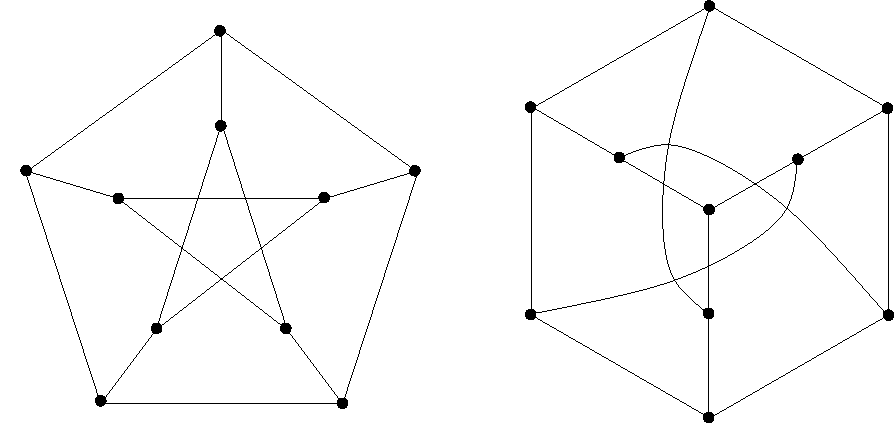
\includegraphics{./petersen_iso.pdf}%
\end{picture}%
\setlength{\unitlength}{3947sp}%
%
\begingroup\makeatletter\ifx\SetFigFont\undefined%
\gdef\SetFigFont#1#2#3#4#5{%
  \reset@font\fontsize{#1}{#2pt}%
  \fontfamily{#3}\fontseries{#4}\fontshape{#5}%
  \selectfont}%
\fi\endgroup%
\begin{picture}(7159,3450)(1453,-8445)
\put(3280,-5177){\makebox(0,0)[lb]{\smash{{\SetFigFont{12}{14.4}{\familydefault}{\mddefault}{\updefault}{\color[rgb]{0,0,0}A}%
}}}}
\put(4846,-6295){\makebox(0,0)[lb]{\smash{{\SetFigFont{12}{14.4}{\familydefault}{\mddefault}{\updefault}{\color[rgb]{0,0,0}B}%
}}}}
\put(4231,-8422){\makebox(0,0)[lb]{\smash{{\SetFigFont{12}{14.4}{\familydefault}{\mddefault}{\updefault}{\color[rgb]{0,0,0}C}%
}}}}
\put(2126,-8430){\makebox(0,0)[lb]{\smash{{\SetFigFont{12}{14.4}{\familydefault}{\mddefault}{\updefault}{\color[rgb]{0,0,0}D}%
}}}}
\put(1468,-6280){\makebox(0,0)[lb]{\smash{{\SetFigFont{12}{14.4}{\familydefault}{\mddefault}{\updefault}{\color[rgb]{0,0,0}E}%
}}}}
\put(3316,-5978){\makebox(0,0)[lb]{\smash{{\SetFigFont{12}{14.4}{\familydefault}{\mddefault}{\updefault}{\color[rgb]{0,0,0}F}%
}}}}
\put(4116,-6756){\makebox(0,0)[lb]{\smash{{\SetFigFont{12}{14.4}{\familydefault}{\mddefault}{\updefault}{\color[rgb]{0,0,0}G}%
}}}}
\put(3839,-7661){\makebox(0,0)[lb]{\smash{{\SetFigFont{12}{14.4}{\familydefault}{\mddefault}{\updefault}{\color[rgb]{0,0,0}H}%
}}}}
\put(2244,-6796){\makebox(0,0)[lb]{\smash{{\SetFigFont{12}{14.4}{\familydefault}{\mddefault}{\updefault}{\color[rgb]{0,0,0}J}%
}}}}
\put(2519,-7663){\makebox(0,0)[lb]{\smash{{\SetFigFont{12}{14.4}{\familydefault}{\mddefault}{\updefault}{\color[rgb]{0,0,0}I}%
}}}}
\end{picture}%


\vspace{.2in}

\item We will use the symbol $\Integers^{\ast}$ to refer to the set of
all integers \emph{except} $0$.  
Define a relation $\relQ$ on the set of all pairs in $\Integers \times \Integers^{\ast}$ (pairs of integers where the second coordinate is non-zero) by
$(a,b) \relQ (c,d) \; \iff \; ad=bc$.  Show that $\relQ$ is an 
equivalence relation.

\item The relation $\relQ$ defined in the previous problem partitions
the set of all pairs of integers into an interesting set of equivalence
classes.  Explain why 

\[ \Rationals \quad = \quad (\Integers \times \Integers^{\ast}) / \relQ. \]

\noindent Ultimately, this is the ``right'' definition of the set 
of rational numbers!

\item Reflect back on the proof in problem 5.  Note that we were fairly
careful in assuring that the second coordinate in the ordered pairs is
non-zero. (This was the whole reason for introducing the 
$\Integers^{\ast}$ notation.)  At what point in the argument did you
use this hypothesis?

\end{enumerate} 

%% Emacs customization
%% 
%% Local Variables: ***
%% TeX-master: "GIAM-hw.tex" ***
%% comment-column:0 ***
%% comment-start: "%% "  ***
%% comment-end:"***" ***
%% End: ***


\newpage

\section{Ordering relations}
\label{sec:ord_rel}

The prototype for ordering relations is $\leq$.  Although a case
could be made for using $<$ as the prototypical ordering relation.  
These two relations differ in one important sense: $\leq$ is reflexive
and $<$ is irreflexive.  Various authors, having made different 
choices as to which of these is the more prototypical, have
defined ordering relations in slightly different ways.  The 
majority view seems to be that an ordering relation is
reflexive (which means that 
ordering relations are modeled after $\leq$).  
We would really like to take the contrary position -- we always
root for the underdog -- but one of our favorite ordering
relation (divisibility) is reflexive and it would be eliminated
if we made the other choice\footnote{If you insist on making the other %
choice, you will have a ``strict ordering relation'' a.k.a. an ``irreflexive %
ordering relation''}.  So\ldots

\begin{defi}
A relation $\relR$ on a set $S$ is an 
\index{ordering relation}\emph{ordering relation}
iff $\relR$ is reflexive, anti-symmetric and transitive.
\end{defi}

Now, we've used $\leq$ to decide what properties an ordering relation
should have, but we should point out that most ordering relations
don't do nearly as good a job as $\leq$ does.  The $\leq$ relation
imposes what is known as a \index{total order}\emph{total order}
on the sets that it acts on (you should note that it can't be used
to compare complex numbers, but it can be placed between reals or
any of the sets of numbers that are contained in $\Reals$.)  Most
ordering relations only create what is known as a \index{partial order}
\emph{partial order} on the sets they act on.  In a total ordering
(a.k.a. a linear ordering) every pair of elements can be compared
and we can use the ordering relation to decide which order they go
in.  In a partial ordering there may be elements that are incomparable.

\begin{defi}
If $x$ and $y$ are elements of a set $S$ and $\relR$ is an ordering
relation on $S$ then we say $x$ and $y$ are \emph{comparable} if
$x\relR y \; \lor \; y\relR x$.
\end{defi}

\begin{defi}
If $x$ and $y$ are elements of a set $S$ and $\relR$ is an ordering
relation on $S$ then we say $x$ and $y$ are \emph{incomparable} if
neither $x\relR y$ nor $y\relR x$ is true.
\end{defi}

Consider the set $S = \{1, 2, 3, 4, 6, 12 \}$.  If we look at the
relation $\leq$ on this set we get the following digraph.

\begin{center}
\begin{picture}(0,0)%
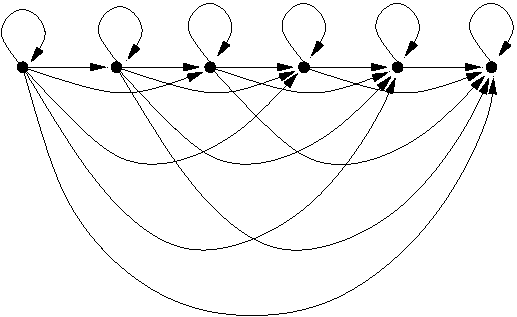
\includegraphics{figures/total_order.pdf}%
\end{picture}%
\setlength{\unitlength}{3947sp}%
%
\begingroup\makeatletter\ifx\SetFigFont\undefined%
\gdef\SetFigFont#1#2#3#4#5{%
  \reset@font\fontsize{#1}{#2pt}%
  \fontfamily{#3}\fontseries{#4}\fontshape{#5}%
  \selectfont}%
\fi\endgroup%
\begin{picture}(4118,2521)(4094,-2960)
\put(5776,-736){\makebox(0,0)[lb]{\smash{{\SetFigFont{12}{14.4}{\familydefault}{\mddefault}{\updefault}{\color[rgb]{0,0,0}3}%
}}}}
\put(5026,-736){\makebox(0,0)[lb]{\smash{{\SetFigFont{12}{14.4}{\familydefault}{\mddefault}{\updefault}{\color[rgb]{0,0,0}2}%
}}}}
\put(4276,-736){\makebox(0,0)[lb]{\smash{{\SetFigFont{12}{14.4}{\familydefault}{\mddefault}{\updefault}{\color[rgb]{0,0,0}1}%
}}}}
\put(6526,-736){\makebox(0,0)[lb]{\smash{{\SetFigFont{12}{14.4}{\familydefault}{\mddefault}{\updefault}{\color[rgb]{0,0,0}4}%
}}}}
\put(7276,-736){\makebox(0,0)[lb]{\smash{{\SetFigFont{12}{14.4}{\familydefault}{\mddefault}{\updefault}{\color[rgb]{0,0,0}6}%
}}}}
\put(7951,-736){\makebox(0,0)[lb]{\smash{{\SetFigFont{12}{14.4}{\familydefault}{\mddefault}{\updefault}{\color[rgb]{0,0,0}12}%
}}}}
\end{picture}%

\end{center}

On the other hand, perhaps you noticed these numbers are the 
divisors of $12$.  The divisibility relation will give us our
first example of a partial order.

\begin{center}
\begin{picture}(0,0)%
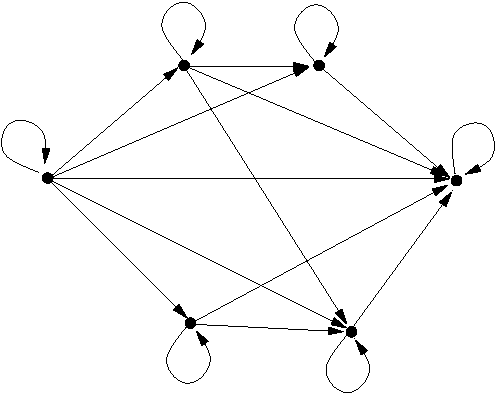
\includegraphics{figures/partial_order.pdf}%
\end{picture}%
\setlength{\unitlength}{3947sp}%
%
\begingroup\makeatletter\ifx\SetFigFont\undefined%
\gdef\SetFigFont#1#2#3#4#5{%
  \reset@font\fontsize{#1}{#2pt}%
  \fontfamily{#3}\fontseries{#4}\fontshape{#5}%
  \selectfont}%
\fi\endgroup%
\begin{picture}(3967,3147)(1243,-3585)
\put(1401,-1638){\makebox(0,0)[lb]{\smash{{\SetFigFont{12}{14.4}{\familydefault}{\mddefault}{\updefault}{\color[rgb]{0,0,0}1}%
}}}}
\put(4926,-1713){\makebox(0,0)[lb]{\smash{{\SetFigFont{12}{14.4}{\familydefault}{\mddefault}{\updefault}{\color[rgb]{0,0,0}12}%
}}}}
\put(2676,-763){\makebox(0,0)[lb]{\smash{{\SetFigFont{12}{14.4}{\familydefault}{\mddefault}{\updefault}{\color[rgb]{0,0,0}2}%
}}}}
\put(3726,-768){\makebox(0,0)[lb]{\smash{{\SetFigFont{12}{14.4}{\familydefault}{\mddefault}{\updefault}{\color[rgb]{0,0,0}4}%
}}}}
\put(2721,-3333){\makebox(0,0)[lb]{\smash{{\SetFigFont{12}{14.4}{\familydefault}{\mddefault}{\updefault}{\color[rgb]{0,0,0}3}%
}}}}
\put(3976,-3388){\makebox(0,0)[lb]{\smash{{\SetFigFont{12}{14.4}{\familydefault}{\mddefault}{\updefault}{\color[rgb]{0,0,0}6}%
}}}}
\end{picture}%

\end{center}

\begin{exer}
Which elements in the above partial order are incomparable?
\end{exer}

A set together with an ordering relation creates a mathematical 
structure known as a \index{partially ordered set}\emph{partially
ordered set}.  Since that is a bit of a mouthful, the abbreviated
form \index{poset}\emph{poset} is actually heard more commonly.  
If one wishes to refer to a poset it is necessary to identify
both the set and the ordering relation.  Thus, if $S$ is a set
and $\relR$ is an ordering relation, we write $(S, \relR)$ to
denote the corresponding poset.  

The digraphs given above for two posets having the same underlying
set provide an existence proof -- the same set may have different 
orders imposed upon it.  They also highlight another issue -- these
digraphs for ordering relations get pretty crowded!  \index{Hasse diagrams}
Hasse diagrams
for posets (named after the famous German mathematician 
\index{Hasse, Helmut}Helmut Hasse) are a way of displaying all the 
information in a poset's digraph, but much more succinctly.  There
are features of a Hasse diagram that correspond to each of the 
properties that an ordering relation must have.  

Since ordering relations are always reflexive, there will always 
be loops at every vertex in the digraph.  In a Hasse diagram we
leave out the loops.

Since ordering relations are anti-symmetric, every edge in the digraph
will go in one direction or the other.  In a Hasse diagram we arrange
the vertices so that that direction is \emph{upward} -- that way we
can leave out all the arrowheads without losing any information.

The final simplification that we make in creating a Hasse diagram for
a poset has to do with the transitivity property -- we leave out any
connections that could be deduced because of transitivity.

Hasse diagrams for the two orderings that we've been discussing are 
shown in Figure~\ref{fig:hasse_diag}


\begin{figure}[!hbt]
\begin{picture}(0,0)%
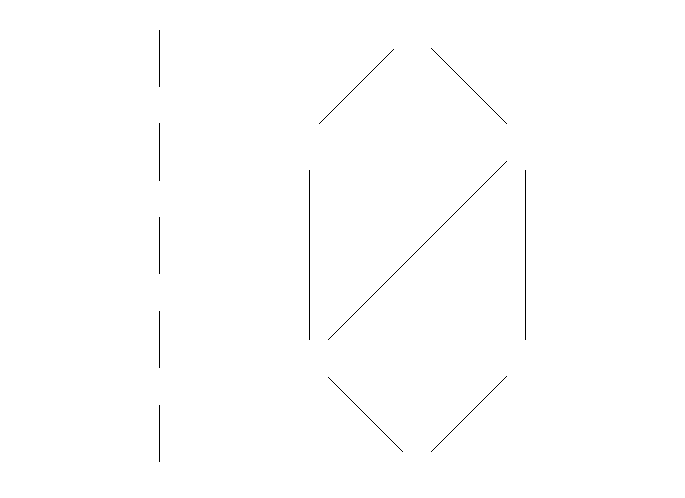
\includegraphics{./Hasse_diagram.pdf}%
\end{picture}%
\setlength{\unitlength}{3947sp}%
%
\begingroup\makeatletter\ifx\SetFigFont\undefined%
\gdef\SetFigFont#1#2#3#4#5{%
  \reset@font\fontsize{#1}{#2pt}%
  \fontfamily{#3}\fontseries{#4}\fontshape{#5}%
  \selectfont}%
\fi\endgroup%
\begin{picture}(5477,3978)(-600,-3730)
\put(626,-661){\makebox(0,0)[lb]{\smash{{\SetFigFont{12}{14.4}{\familydefault}{\mddefault}{\updefault}{\color[rgb]{0,0,0}$6$}%
}}}}
\put(596, 89){\makebox(0,0)[lb]{\smash{{\SetFigFont{12}{14.4}{\familydefault}{\mddefault}{\updefault}{\color[rgb]{0,0,0}$12$}%
}}}}
\put(636,-3661){\makebox(0,0)[lb]{\smash{{\SetFigFont{12}{14.4}{\familydefault}{\mddefault}{\updefault}{\color[rgb]{0,0,0}$1$}%
}}}}
\put(626,-2901){\makebox(0,0)[lb]{\smash{{\SetFigFont{12}{14.4}{\familydefault}{\mddefault}{\updefault}{\color[rgb]{0,0,0}$2$}%
}}}}
\put(636,-2161){\makebox(0,0)[lb]{\smash{{\SetFigFont{12}{14.4}{\familydefault}{\mddefault}{\updefault}{\color[rgb]{0,0,0}$3$}%
}}}}
\put(646,-1411){\makebox(0,0)[lb]{\smash{{\SetFigFont{12}{14.4}{\familydefault}{\mddefault}{\updefault}{\color[rgb]{0,0,0}$4$}%
}}}}
\put(2701,-3586){\makebox(0,0)[lb]{\smash{{\SetFigFont{12}{14.4}{\familydefault}{\mddefault}{\updefault}{\color[rgb]{0,0,0}$1$}%
}}}}
\put(1876,-2686){\makebox(0,0)[lb]{\smash{{\SetFigFont{12}{14.4}{\familydefault}{\mddefault}{\updefault}{\color[rgb]{0,0,0}$2$}%
}}}}
\put(3526,-2686){\makebox(0,0)[lb]{\smash{{\SetFigFont{12}{14.4}{\familydefault}{\mddefault}{\updefault}{\color[rgb]{0,0,0}$3$}%
}}}}
\put(1876,-961){\makebox(0,0)[lb]{\smash{{\SetFigFont{12}{14.4}{\familydefault}{\mddefault}{\updefault}{\color[rgb]{0,0,0}$4$}%
}}}}
\put(3526,-961){\makebox(0,0)[lb]{\smash{{\SetFigFont{12}{14.4}{\familydefault}{\mddefault}{\updefault}{\color[rgb]{0,0,0}$6$}%
}}}}
\put(2626,-61){\makebox(0,0)[lb]{\smash{{\SetFigFont{12}{14.4}{\familydefault}{\mddefault}{\updefault}{\color[rgb]{0,0,0}$12$}%
}}}}
\end{picture}%

\caption[Some simple Hasse diagrams.]{Hasse diagrams of the set $\{1,2,3,4,6,12\}$ %
totally ordered by $\leq$ and partially ordered by $\mid$.}
\label{fig:hasse_diag} 
\end{figure}

Often there is some feature of the elements of the set being ordered
that allows us to arrange a Hasse diagram in ``ranks.''  For example,
consider ${\mathcal P}(\{1,2,3\})$, the set of all subsets of a three
element set -- this set can be partially ordered using the $\subseteq$ 
relation.  (Technically, we should verify that this relation is reflexive,
anti-symmetric and transitive before proceeding, but by now you know
why subset containment is denoted using a rounded version of $\leq$.)
Subsets of the same size can't possibly be included one in the other
unless they happen to be equal!  This allows us to draw the Hasse 
diagram for this set with the nodes arranged in four rows. 
(See Figure~\ref{fig:subset_hasse}.)  

\begin{figure}[!hbtp]
\begin{picture}(0,0)%
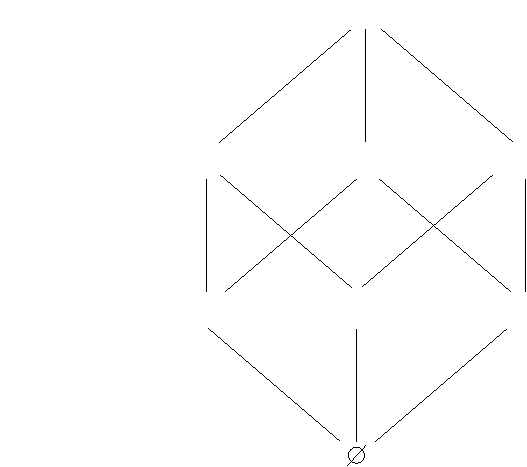
\includegraphics{./Hasse_for_subsets.pdf}%
\end{picture}%
\setlength{\unitlength}{3947sp}%
%
\begingroup\makeatletter\ifx\SetFigFont\undefined%
\gdef\SetFigFont#1#2#3#4#5{%
  \reset@font\fontsize{#1}{#2pt}%
  \fontfamily{#3}\fontseries{#4}\fontshape{#5}%
  \selectfont}%
\fi\endgroup%
\begin{picture}(4213,3724)(3300,-3938)
\put(4801,-2761){\makebox(0,0)[lb]{\smash{{\SetFigFont{12}{14.4}{\rmdefault}{\mddefault}{\updefault}{\color[rgb]{0,0,0}$\{1\}$}%
}}}}
\put(6001,-2761){\makebox(0,0)[lb]{\smash{{\SetFigFont{12}{14.4}{\rmdefault}{\mddefault}{\updefault}{\color[rgb]{0,0,0}$\{2\}$}%
}}}}
\put(7201,-2761){\makebox(0,0)[lb]{\smash{{\SetFigFont{12}{14.4}{\rmdefault}{\mddefault}{\updefault}{\color[rgb]{0,0,0}$\{3\}$}%
}}}}
\put(7126,-1561){\makebox(0,0)[lb]{\smash{{\SetFigFont{12}{14.4}{\rmdefault}{\mddefault}{\updefault}{\color[rgb]{0,0,0}$\{2,3\}$}%
}}}}
\put(5926,-1561){\makebox(0,0)[lb]{\smash{{\SetFigFont{12}{14.4}{\rmdefault}{\mddefault}{\updefault}{\color[rgb]{0,0,0}$\{1,3\}$}%
}}}}
\put(4726,-1561){\makebox(0,0)[lb]{\smash{{\SetFigFont{12}{14.4}{\rmdefault}{\mddefault}{\updefault}{\color[rgb]{0,0,0}$\{1,2\}$}%
}}}}
\put(5851,-361){\makebox(0,0)[lb]{\smash{{\SetFigFont{12}{14.4}{\rmdefault}{\mddefault}{\updefault}{\color[rgb]{0,0,0}$\{1,2,3\}$}%
}}}}
\end{picture}%

\caption[Hasse diagram for $({\mathcal P}(\{1,2,3\}), \subseteq)$.]{Hasse %
diagram for the power set of $\{1,2,3\}$ partially ordered by %
set containment.}
\label{fig:subset_hasse} 
\end{figure}

\begin{exer}
Try drawing a Hasse diagram for the partially ordered set 

\[ ({\mathcal P}(\{1,2,3,4\}),\subseteq). \]

\end{exer}


Posets like $({\mathcal P}(\{1,2,3\}), \subseteq)$ that can be laid out
in ranks are known as \index{graded poset} \emph{graded posets}.  Things
in a graded poset that have the same rank are always incomparable.

\begin{defi}
A \emph{graded poset} is a triple $(S, \relR, \rho)$, where $S$ is a set,
$\relR$ is an ordering relation, and $\rho$ is a function from $S$ to $\Integers$.
\end{defi}

In the example we've been considering (the graded poset of subsets of a set
partially ordered by set inclusion), the grading function $\rho$ takes a
subset to its size.  That is, $\rho(A) = |A|$.  Another nice example of
a graded poset is the set of divisors of some number partially ordered
by the divisibility relation ($\mid$).  In this case the grading function
takes a number to its total degree -- the sum of all the exponents
appearing in its prime factorization.  In Figure~\ref{fig:divisors_of_72}
we show the poset of divisors of $72$ and indicate the grading.

\begin{figure}[!hbtp]
\begin{picture}(0,0)%
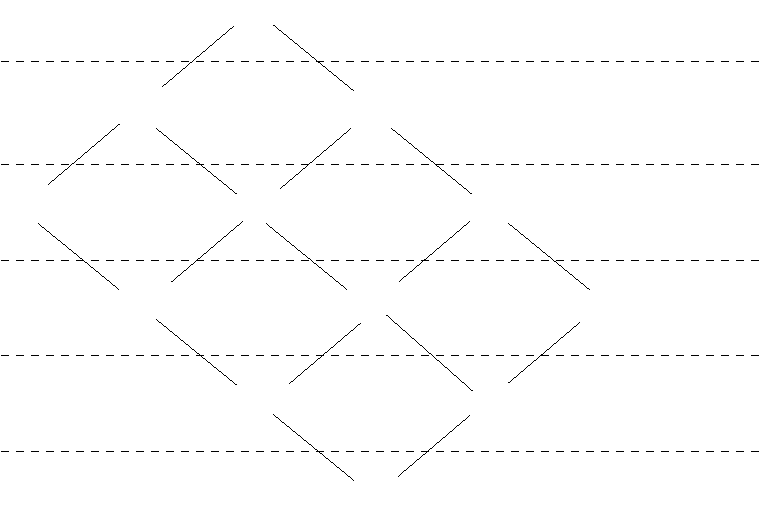
\includegraphics{./divisors_of_72.pdf}%
\end{picture}%
\setlength{\unitlength}{3947sp}%
%
\begingroup\makeatletter\ifx\SetFigFont\undefined%
\gdef\SetFigFont#1#2#3#4#5{%
  \reset@font\fontsize{#1}{#2pt}%
  \fontfamily{#3}\fontseries{#4}\fontshape{#5}%
  \selectfont}%
\fi\endgroup%
\begin{picture}(6138,4118)(1039,-4766)
\put(6754,-4711){\makebox(0,0)[lb]{\smash{{\SetFigFont{12}{14.4}{\rmdefault}{\mddefault}{\updefault}{\color[rgb]{0,0,0}$0$}%
}}}}
\put(6754,-3888){\makebox(0,0)[lb]{\smash{{\SetFigFont{12}{14.4}{\rmdefault}{\mddefault}{\updefault}{\color[rgb]{0,0,0}$1$}%
}}}}
\put(6754,-3123){\makebox(0,0)[lb]{\smash{{\SetFigFont{12}{14.4}{\rmdefault}{\mddefault}{\updefault}{\color[rgb]{0,0,0}$2$}%
}}}}
\put(6754,-2359){\makebox(0,0)[lb]{\smash{{\SetFigFont{12}{14.4}{\rmdefault}{\mddefault}{\updefault}{\color[rgb]{0,0,0}$3$}%
}}}}
\put(6754,-1535){\makebox(0,0)[lb]{\smash{{\SetFigFont{12}{14.4}{\rmdefault}{\mddefault}{\updefault}{\color[rgb]{0,0,0}$4$}%
}}}}
\put(6754,-771){\makebox(0,0)[lb]{\smash{{\SetFigFont{12}{14.4}{\rmdefault}{\mddefault}{\updefault}{\color[rgb]{0,0,0}$5$}%
}}}}
\put(2874,-771){\makebox(0,0)[lb]{\smash{{\SetFigFont{12}{14.4}{\rmdefault}{\mddefault}{\updefault}{\color[rgb]{0,0,0}$72=2^3\cdot3^2$}%
}}}}
\put(1991,-1535){\makebox(0,0)[lb]{\smash{{\SetFigFont{12}{14.4}{\rmdefault}{\mddefault}{\updefault}{\color[rgb]{0,0,0}$24=2^3\cdot3^1$}%
}}}}
\put(3814,-1535){\makebox(0,0)[lb]{\smash{{\SetFigFont{12}{14.4}{\rmdefault}{\mddefault}{\updefault}{\color[rgb]{0,0,0}$36=2^2\cdot3^2$}%
}}}}
\put(4755,-2359){\makebox(0,0)[lb]{\smash{{\SetFigFont{12}{14.4}{\rmdefault}{\mddefault}{\updefault}{\color[rgb]{0,0,0}$18=2^1\cdot3^2$}%
}}}}
\put(2933,-2359){\makebox(0,0)[lb]{\smash{{\SetFigFont{12}{14.4}{\rmdefault}{\mddefault}{\updefault}{\color[rgb]{0,0,0}$12=2^2\cdot3^1$}%
}}}}
\put(1110,-2359){\makebox(0,0)[lb]{\smash{{\SetFigFont{12}{14.4}{\rmdefault}{\mddefault}{\updefault}{\color[rgb]{0,0,0}$8=2^3$}%
}}}}
\put(2051,-3123){\makebox(0,0)[lb]{\smash{{\SetFigFont{12}{14.4}{\rmdefault}{\mddefault}{\updefault}{\color[rgb]{0,0,0}$4=2^2$}%
}}}}
\put(3873,-3123){\makebox(0,0)[lb]{\smash{{\SetFigFont{12}{14.4}{\rmdefault}{\mddefault}{\updefault}{\color[rgb]{0,0,0}$6=2^1\cdot3^1$}%
}}}}
\put(5716,-3156){\makebox(0,0)[lb]{\smash{{\SetFigFont{12}{14.4}{\rmdefault}{\mddefault}{\updefault}{\color[rgb]{0,0,0}$9=3^2$}%
}}}}
\put(4873,-3888){\makebox(0,0)[lb]{\smash{{\SetFigFont{12}{14.4}{\rmdefault}{\mddefault}{\updefault}{\color[rgb]{0,0,0}$3^1$}%
}}}}
\put(2991,-3888){\makebox(0,0)[lb]{\smash{{\SetFigFont{12}{14.4}{\rmdefault}{\mddefault}{\updefault}{\color[rgb]{0,0,0}$2^1$}%
}}}}
\put(3931,-4652){\makebox(0,0)[lb]{\smash{{\SetFigFont{12}{14.4}{\rmdefault}{\mddefault}{\updefault}{\color[rgb]{0,0,0}$1$}%
}}}}
\end{picture}%

\caption[Hasse diagram of divisors of 72.]{Hasse %
diagram for the divisors of $72$, partially ordered by %
divisibility. This is a graded poset.}
\label{fig:divisors_of_72} 
\end{figure}

We will end this section by giving a small collection of terminology
relevant to partially ordered sets.

A \index{chain}\emph{chain} in a poset is a subset of the elements, all 
of which are comparable.  If you restrict your attention to a chain within 
a poset, you will be looking at a total order.  
An \index{antichain}\emph{antichain} in a poset is a subset
of the elements, none of which are comparable.  Thus, for example, a subset
of elements having the same rank (in a graded poset) is an antichain.  
Chains and antichains are said to be \emph{maximal} if it
is not possible to add further elements to them (whilst maintaining the 
properties that make them chains and/or antichains).  An element $x$, that 
appears above another element $y$ -- and connected to it -- in a Hasse
diagram is said to \index{cover, in a poset}\emph{cover} it.  In this situation
you may also say that $x$ is an \index{successor}\emph{immediate successor} of
$y$.  A \index{maximal element, in a poset}\emph{maximal element} is an element that is not covered by any other element.  Similarly, a 
\index{minimal element, in a poset}\emph{minimal element} is an element that is not a cover of any other element.  If a chain is maximal, it follows that it
must contain both a maximal and a minimal element (with respect to the
surrounding poset).  The collection of all maximal elements forms an antichain,
as does (separately) the collection of all minimal elements.  Finally,
we have the notions of \index{greatest element, in a poset} 
\emph{greatest element} (a.k.a. \index{top, in a poset}top) and 
\index{least element, in a poset}\emph{least element} (a.k.a. 
\index{bottom, in a poset}bottom) -- the greatest element is greater than every
other element in the poset,  the least element is smaller than every other element.  Please be careful to distinguish these
concepts from maximal and minimal elements -- a greatest element is 
automatically maximal, and a least element is always minimal, but it 
is possible to have a poset with no greatest element that nevertheless 
has one or more maximal elements, and it is possible to have a poset with no
least element that has one or more minimal elements. 

In the poset of divisors of $72$, the subset $\{2, 6, 12, 24\}$ is a chain.  
Since it would be possible to add both $1$ and $72$ to this chain and still 
have a chain, this chain is not maximal.  (But, of course, 
$\{1, 2, 6, 12, 24, 72\}$ is.)  On the other hand, 
$\{8, 12, 18\}$ is an antichain (indeed, this is a maximal antichain).  
This poset has both a top and a bottom -- $1$ is the least element
and $72$ is the greatest element.   Notice that the elements which cover
$1$ (the least element) are the prime divisors of $72$.

\newpage

\noindent{\large \bf Exercises --- \thesection\ }

\begin{enumerate}
\item In population ecology there is a partial order ``predates''
which basically means that one organism feeds upon another.  Strictly
speaking this relation is not transitive; however, if we take the point
of view that when a wolf eats a sheep, it is also eating some of the grass
that the sheep has fed upon, we see that in a certain sense it is transitive.
A chain in this partial order is called a ``food chain'' and so-called 
apex predators are said to ``sit atop the food chain''.  Thus ``apex 
predator'' is a term for a maximal element in this poset.   When poisons
such as mercury and PCBs are introduced into an ecosystem, they tend to
collect disproportionately in the apex predators -- which is why pregnant
women and young children should not eat shark or tuna but sardines 
are fine.

Below is a small example of an ecology partially ordered by ``predates''

\begin{center}
\begin{picture}(0,0)%
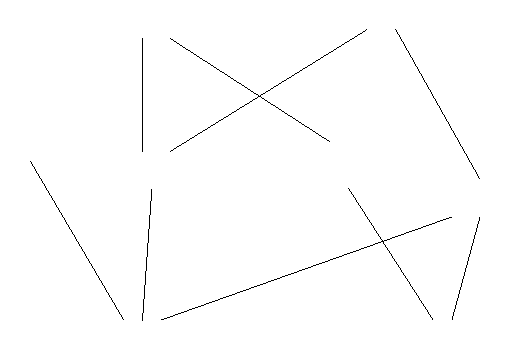
\includegraphics{./ecosystem.pdf}%
\end{picture}%
\setlength{\unitlength}{3947sp}%
%
\begingroup\makeatletter\ifx\SetFigFont\undefined%
\gdef\SetFigFont#1#2#3#4#5{%
  \reset@font\fontsize{#1}{#2pt}%
  \fontfamily{#3}\fontseries{#4}\fontshape{#5}%
  \selectfont}%
\fi\endgroup%
\begin{picture}(4091,2787)(1786,-3376)
\put(2874,-771){\makebox(0,0)[lb]{\smash{{\SetFigFont{12}{14.4}{\rmdefault}{\mddefault}{\updefault}{\color[rgb]{0,0,0}Fox}%
}}}}
\put(4651,-736){\makebox(0,0)[lb]{\smash{{\SetFigFont{12}{14.4}{\rmdefault}{\mddefault}{\updefault}{\color[rgb]{0,0,0}Alligator}%
}}}}
\put(1801,-1786){\makebox(0,0)[lb]{\smash{{\SetFigFont{12}{14.4}{\rmdefault}{\mddefault}{\updefault}{\color[rgb]{0,0,0}Cow}%
}}}}
\put(5401,-2236){\makebox(0,0)[lb]{\smash{{\SetFigFont{12}{14.4}{\rmdefault}{\mddefault}{\updefault}{\color[rgb]{0,0,0}Goose}%
}}}}
\put(2851,-2011){\makebox(0,0)[lb]{\smash{{\SetFigFont{12}{14.4}{\rmdefault}{\mddefault}{\updefault}{\color[rgb]{0,0,0}Duck}%
}}}}
\put(4276,-1936){\makebox(0,0)[lb]{\smash{{\SetFigFont{12}{14.4}{\rmdefault}{\mddefault}{\updefault}{\color[rgb]{0,0,0}Robin}%
}}}}
\put(5101,-3361){\makebox(0,0)[lb]{\smash{{\SetFigFont{12}{14.4}{\rmdefault}{\mddefault}{\updefault}{\color[rgb]{0,0,0}Worms}%
}}}}
\put(2701,-3361){\makebox(0,0)[lb]{\smash{{\SetFigFont{12}{14.4}{\rmdefault}{\mddefault}{\updefault}{\color[rgb]{0,0,0}Grass}%
}}}}
\end{picture}%

\end{center}

Find the largest antichain in this poset.

\newpage

\item Referring to the poset given in exercise 1, match the following.

\begin{tabular}{lr}
\rule{2.3in}{0pt} & \rule{2.3in}{0pt} \\
\begin{minipage}[b]{.4\textwidth}
\begin{enumerate}
\item[1.] An (non-maximal) antichain
\item[2.] A maximal antichain
\item[3.] A maximal element
\item[4.] A (non-maximal) chain
\item[5.] A maximal chain
\item[6.] A cover for ``Worms''
\item[7.] A least element
\item[8.] A minimal element
\end{enumerate}
\end{minipage} 
 & 
\begin{minipage}[b]{.4\textwidth}
\begin{enumerate}
\item[a.] Grass 
\item[b.] Goose
\item[c.] Fox
\item[d.] $\{ \mbox{Grass}, \mbox{Duck} \}$
\item[e.] There isn't one!
\item[f.] $\{ \mbox{Fox}, \mbox{Alligator}, \mbox{Cow} \}$
\item[g.] $\{ \mbox{Cow}, \mbox{Duck}, \mbox{Robin}, \mbox{Goose} \}$
\item[h.] $\{ \mbox{Worms}, \mbox{Robin}, \mbox{Fox} \}$
\end{enumerate} 
\end{minipage} \\
\end{tabular}

\item The graph of the edges of a cube is one in an infinite sequence of 
graphs.  These graphs are defined 
recursively by ``Make two copies of the previous graph then join 
corresponding nodes in the two copies with edges.''  The $0$-dimensional
`cube' is just a single point.  The $1$-dimensional cube is a single edge
with a node at either end.  The $2$-dimensional cube is actually a square
and the $3$-dimensional cube is what we usually mean when we say ``cube.''

\begin{center}
\begin{picture}(0,0)%
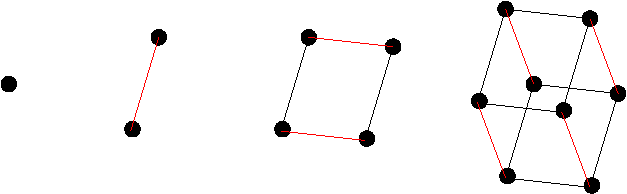
\includegraphics{./0-3_dim_cubes.pdf}%
\end{picture}%
\setlength{\unitlength}{3947sp}%
%
\begingroup\makeatletter\ifx\SetFigFont\undefined%
\gdef\SetFigFont#1#2#3#4#5{%
  \reset@font\fontsize{#1}{#2pt}%
  \fontfamily{#3}\fontseries{#4}\fontshape{#5}%
  \selectfont}%
\fi\endgroup%
\begin{picture}(5015,1548)(1656,-6190)
\end{picture}%

\end{center}

Make a careful drawing of a \index{hypercube}\emph{hypercube} -- which is
the name of the graph that follows the ordinary cube in this sequence.

\item Label the nodes of a hypercube with the divisors of $210$ in order to
produce a Hasse diagram of the poset determined by the divisibility relation.

\item Label the nodes of a hypercube with the subsets of $\{a,b,c,d\}$ 
in order to produce a Hasse diagram of the poset determined by the 
subset containment relation.
  
\item Complete a Hasse diagram for the poset of divisors of 11025 (partially ordered by divisibility).

\item Find a collection of sets so that, when they are partially ordered by $\subseteq$, we obtain the same Hasse diagram as in the previous problem.

\end{enumerate}

%% Emacs customization
%% 
%% Local Variables: ***
%% TeX-master: "GIAM-hw.tex" ***
%% comment-column:0 ***
%% comment-start: "%% "  ***
%% comment-end:"***" ***
%% End: ***


\newpage

\section{Functions}
\label{sec:functions}

The concept of a function is one of the most useful abstractions
in mathematics.  In fact it is an abstraction that can be further
abstracted!  For instance an \index{operator}\emph{operator} 
is an entity which takes functions as inputs and produces functions
as outputs, thus an operator is to functions as functions themselves
are to numbers.  There are many operators that you have certainly
encountered already -- just not by that name.  One of the most
famous operators is ``differentiation,'' when you take the derivative
of some function, the answer you obtain is another function.  
If two different people are given the same differentiation problem
and they come up with different answers, we \emph{know} that at least
one of them has made a mistake!  Similarly, if two calculations of the
value of a function are made for the same input, they \emph{must} match.

The property we are discussing used to be captured by saying that a 
function needs to be ``well-defined.''  The old school definition of a 
function was: 

\begin{defi}
 A \emph{function} $f$ is a well-defined rule, that, given any input
value $x$ produces a unique output\footnote{The use of the notation %
$f(x)$ to indicate the output of function $f$ associated with input $x$ %
was instituted by Leonard Euler, and so it is known as Euler notation.} 
value $f(x)$.
\end{defi}

A more modern definition of a function is the following.

\begin{defi}
 A \emph{function} is a binary relation which does not contain
distinct pairs having the same initial element.
\end{defi}

When we think of a function as a special type of binary relation, 
the pairs that are ``in'' the function have the form $(x, f(x))$,
that is, they consist of an input and the corresponding output.

We have gotten relatively used to relations ``on'' a set, but recall
that the more general situation is that a binary relation is 
a subset of $A \times B$.  In this setting, if the relation is 
actually a function $f$, we say that $f$ is a function \emph{from} $A$
\emph{to} $B$.  Now, quite often there are input values  that simply don't 
work for a given function (for instance the well-known ``you can't take
the square root of a negative'' rule).  Also, it is often the case that
certain outputs just can't happen.  So, when dealing with a function
as a relation contained in $A \times B$ there are actually four sets
that are of interest -- the sets $A$ and $B$ (of course) but also some
sets that we'll denote by $A'$ and $B'$.  The set $A'$ consists of those
elements of $A$ that actually appear as the first coordinate of a pair
in the relation $f$.  The set $B'$ consists of those elements of $B$
that actually appear as the second coordinate of a pair in the relation $f$.
A generic example of how these four sets might look is given in Figure~\ref{fig:generic_function}.

\begin{figure}[!hbtp]
\begin{picture}(0,0)%
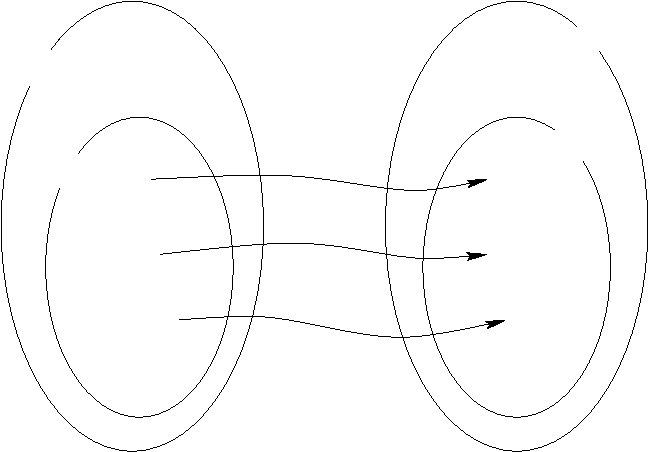
\includegraphics{figures/generic_function.pdf}%
\end{picture}%
\setlength{\unitlength}{3947sp}%
%
\begingroup\makeatletter\ifx\SetFigFont\undefined%
\gdef\SetFigFont#1#2#3#4#5{%
  \reset@font\fontsize{#1}{#2pt}%
  \fontfamily{#3}\fontseries{#4}\fontshape{#5}%
  \selectfont}%
\fi\endgroup%
\begin{picture}(5191,3614)(2018,-5693)
\put(2851,-2386){\makebox(0,0)[lb]{\smash{{\SetFigFont{12}{14.4}{\rmdefault}{\mddefault}{\updefault}{\color[rgb]{0,0,0}$a$}%
}}}}
\put(3151,-2761){\makebox(0,0)[lb]{\smash{{\SetFigFont{12}{14.4}{\rmdefault}{\mddefault}{\updefault}{\color[rgb]{0,0,0}$b$}%
}}}}
\put(3001,-3586){\makebox(0,0)[lb]{\smash{{\SetFigFont{12}{14.4}{\rmdefault}{\mddefault}{\updefault}{\color[rgb]{0,0,0}$c$}%
}}}}
\put(3076,-4186){\makebox(0,0)[lb]{\smash{{\SetFigFont{12}{14.4}{\rmdefault}{\mddefault}{\updefault}{\color[rgb]{0,0,0}$d$}%
}}}}
\put(3226,-4711){\makebox(0,0)[lb]{\smash{{\SetFigFont{12}{14.4}{\rmdefault}{\mddefault}{\updefault}{\color[rgb]{0,0,0}$e$}%
}}}}
\put(6001,-2461){\makebox(0,0)[lb]{\smash{{\SetFigFont{12}{14.4}{\rmdefault}{\mddefault}{\updefault}{\color[rgb]{0,0,0}$v$}%
}}}}
\put(6001,-2761){\makebox(0,0)[lb]{\smash{{\SetFigFont{12}{14.4}{\rmdefault}{\mddefault}{\updefault}{\color[rgb]{0,0,0}$w$}%
}}}}
\put(6001,-3511){\makebox(0,0)[lb]{\smash{{\SetFigFont{12}{14.4}{\rmdefault}{\mddefault}{\updefault}{\color[rgb]{0,0,0}$x=f(c)$}%
}}}}
\put(6001,-4111){\makebox(0,0)[lb]{\smash{{\SetFigFont{12}{14.4}{\rmdefault}{\mddefault}{\updefault}{\color[rgb]{0,0,0}$y=f(d)$}%
}}}}
\put(6151,-4636){\makebox(0,0)[lb]{\smash{{\SetFigFont{12}{14.4}{\rmdefault}{\mddefault}{\updefault}{\color[rgb]{0,0,0}$z=f(e)$}%
}}}}
\put(2476,-3511){\makebox(0,0)[lb]{\smash{{\SetFigFont{12}{14.4}{\rmdefault}{\mddefault}{\updefault}{\color[rgb]{0,0,0}$A'$}%
}}}}
\put(2251,-2686){\makebox(0,0)[lb]{\smash{{\SetFigFont{12}{14.4}{\rmdefault}{\mddefault}{\updefault}{\color[rgb]{0,0,0}$A$}%
}}}}
\put(6676,-2461){\makebox(0,0)[lb]{\smash{{\SetFigFont{12}{14.4}{\rmdefault}{\mddefault}{\updefault}{\color[rgb]{0,0,0}$B$}%
}}}}
\put(6526,-3286){\makebox(0,0)[lb]{\smash{{\SetFigFont{12}{14.4}{\rmdefault}{\mddefault}{\updefault}{\color[rgb]{0,0,0}$B'$}%
}}}}
\end{picture}%

\caption{The sets related to an arbitrary function.}
\label{fig:generic_function} 
\end{figure}

Sadly, only three of the sets we have just discussed are known to
the mathematical world.  The set we have denoted $A'$ is called the
\emph{domain} of the function $f$.  The set we have denoted $B'$ is 
known as the \emph{range} of the function $f$.  The set we have denoted
$B$ is called the \emph{codomain} of the function $f$.  The set we 
have been calling $A$ does not have a name.  In fact, the formal
definition of the term ``function'' has been rigged so that there
is no difference between the sets $A$ and $A'$.  This seems a shame,
if you think of range and domain as being primary, doesn't it seem
odd that we have a way to refer to a superset of the range (i.e. the 
codomain) but no way of referring to a superset of the domain?

Nevertheless, this is just the way it is \ldots  There is only one
set on the input side -- the domain of our function. 

The domain of
any relation is expressed by writing $\Dom{\relR}$. Which is 
defined as follows.

\begin{defi}
If $\relR$ is a relation from $A$ to $B$ then $\Dom{\relR}$ is
a subset of $A$ defined by

\[ \Dom{\relR} = \{a \in A \suchthat \exists b \in B, (a,b) \in \relR \} 
\]

\end{defi}

We should point out that the notation just given for the domain of a 
relation $\relR$, ($\Dom{\relR}$) has analogs for the other 
sets that are involved with a relation.  We write $\Cod{\relR}$
to refer the the codomain of the relation, and $\Rng{\relR}$
to refer to the range. 

Since we are now thinking of functions as special classes of relations, it follows that a function is just 
a set of ordered pairs.  This means that the identity of a function is
tied up, not just with a formula that gives the output for a given input,
but also with what values can be used for those inputs.   Thus the function
$f(x)=2x$ defined on $\Reals$ is a completely different animal from 
the function $f(x)=2x$ defined on $\Naturals$.  If you really want to
specify a function precisely you must give its domain as well as a 
formula for it.  Usually, one does this by writing a formula, then a 
semicolon, then the domain.  (E.g. $f(x)=x^2; \quad x \geq 0$.)

Okay, so, finally, we are prepared to give the real
definition of a function.

\begin{defi}
If $A$ and $B$ are sets, then $f$ is a function from $A$ to $B$ (which
is expressed symbolically by $f:A\longrightarrow B$), if and only if
$f$ is a subset of $A\times B$, $\Dom{f}=A$ and $((a,b) \in f \; \land \; (a,c) \in f \; \implies \; b=c$.
\end{defi}

Recapping, a function \emph{must} have its domain equal to the set $A$
where its inputs come from.  This is sometimes expressed by saying that
a function is \emph{defined} on its domain.  A function's range and codomain
may be different however.  In the event that the range and codomain \emph{are}
the same ($\Cod{\relR} = \Rng{\relR}$)
we have a rather special situation and the function is graced by
the appellation ``surjection.''  The term ``onto'' is also commonly used
to describe a surjective function.  

\begin{exer}
There is an expression in mathematics, ``Every function is onto its %
range.'' that really doesn't say very much.  Why not?
\end{exer}

If one has elements $x$ and $y$, of the domain and codomain, (respectively)
and $y = f(x)$\footnote{Or, equivalently, $(x,y) \in f$.} then one may 
say that ``$y$ is the image of $x$'' or that
``$x$ is a preimage of $y$.''  Take careful note of the articles used in
these phrases -- we say  ``$y$ is {\bf the} image of $x$'' but 
``$x$ is {\bf a} preimage of $y$.''  This is because $y$ is uniquely determined
by $x$, but not vice versa.  For example, since the squares of $2$ and $-2$ are
both $4$, if we consider the function $f(x) = x^2$, the image of (say) $2$ 
is $4$, but a preimage for $4$ could be either $2$ or $-2$.

It would be pleasant if there were a nice way to refer to the preimage of
some element, $y$, of the range.  One notation that you have probably 
seen before is ``$f^{-1}(y)$.''  There is a major difficulty with writing 
down such a thing.  By writing ``$f^{-1}$'' you are making a rather
vast presumption -- that there actually is a function that serves as an
inverse for $f$.  Usually, there is not.  

One can define an inverse for any relation, the inverse is formed by
simply exchanging the elements in the ordered pairs that make up $\relR$.

\begin{defi}
The \index{inverse relation}\emph{inverse relation} of a relation $\relR$
is denoted $\relR^{-1}$ and 

\[ \relR^{-1} = \{ (y,x) \suchthat (x,y) \in \relR \}. \]
\end{defi}

In terms of graphs, the inverse and the original relation are related
by being reflections in the line $y=x$.  It is possible for one, both,
or neither of these to be functions.  The canonical example to keep
in mind is probably $f(x) = x^2$ and its inverse.

\begin{center}
\begin{picture}(0,0)%
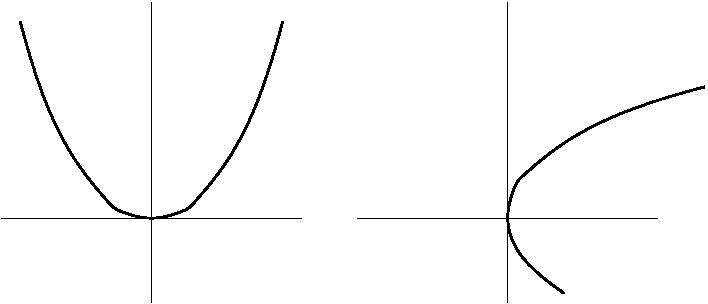
\includegraphics{./square_n_squareroot.pdf}%
\end{picture}%
\setlength{\unitlength}{3947sp}%
%
\begingroup\makeatletter\ifx\SetFigFont\undefined%
\gdef\SetFigFont#1#2#3#4#5{%
  \reset@font\fontsize{#1}{#2pt}%
  \fontfamily{#3}\fontseries{#4}\fontshape{#5}%
  \selectfont}%
\fi\endgroup%
\begin{picture}(5659,2424)(2389,-2773)
\end{picture}%

\end{center}

The graph that we obtain by reflecting $y=f(x)=x^2$ in the line $y=x$ doesn't
pass the vertical line test and so it is the graph of (merely) a relation 
-- not of a function.  The function $g(x) = \sqrt{x}$ that we all know 
and love is not truly the inverse of $f(x)$.  In fact this function is
defined to make a specific (and natural) choice -- it returns the positive
square root of a number.  But this leads to a subtle problem; if we start
with a negative number (say $-3$) and square it we get a positive number ($9$)
and if we then come along and take the square root we get another positive
number ($3$).  This is problematic since we didn't end up where we started
which is what ought to happen if we apply a function followed by its inverse.

We'll try to handle the general situation in a bit, but for the moment let's
consider the nice case: when the inverse of a function is also a function. 
When exactly does this happen?  Well, we have just seen that the inverse
of a function doesn't necessarily pass the vertical line test, and it turns
out that that is the predominant issue.  So, under what circumstances does
the inverse pass the vertical line test?  When the original function 
passes the so-called horizontal line test (every horizontal line
intersects the graph at most once).  Thinking again about $f(x)=x^2$, there
are some horizontal lines that miss the graph entirely, but all horizontal
lines of the form $y=c$ where $c$ is positive will intersect the graph twice.
There are many functions that \emph{do} pass the horizontal line test, for 
instance, consider $f(x) = x^3$.  Such functions are known as 
\index{injection}\emph{injections}, this is the same thing as 
saying a function is ``one-to-one.''   Injective functions can be inverted --
the domain of the inverse function of $f$ will only be the range, $\Rng{f}$,
which as we have seen may fall short of the being the entire codomain, since 
$\Rng{f} \subseteq \Cod{f}$.

Let's first define injections in a way that is divorced from thinking
about their graphs.

\begin{defi}
A function $f(x)$ is an \emph{injection} iff for all pairs of 
inputs $x_1$ and $x_2$, if $f(x_1) = f(x_2)$ then $x_1=x_2$.
\end{defi}

This is another of those defining properties that is designed so
that when it is true it is vacuously true.  An injective function
never takes two distinct inputs to the same output.  Perhaps the 
cleanest way to think about injective functions is in terms of 
preimages -- when a function is injective, preimages are unique.
Actually, this is a good time to mention something about surjective
functions and preimages -- if a function is surjective, every element
of the codomain \emph{has} a preimage.  So, if a function has both 
of these properties it means that every element of the codomain
has one (and only one) preimage.   

A function that is both injective and surjective (one-to-one and onto)
is known as a \index{bijection}\emph{bijection}.  Bijections are tremendously
important in mathematics since they provide a way of perfectly matching
up the elements of two sets.  You will probably spend a good bit of time 
in the future devising maps between sets and then proving that they are
bijections, so we will start practicing that skill now\ldots  

Ordinarily, we will show that a function is a bijection by proving 
separately that it is both a surjection and an injection.  
   
To show that a function is surjective we need to show that it is 
possible to find a preimage for every element of the codomain.  If
we happen to know what the inverse function is, then it is easy to
find a preimage for an arbitrary element.  In terms of the taxonomy
for proofs that was introduced in Chapter~\ref{ch:proof1}, we are talking
about a constructive proof of an existential statement.  A function $f$
is surjective iff $\forall y \in \Cod{f}, \exists x \in \Dom{f}, 
y = f(x)$, so to prove surjectivity is to find the $x$ that ``works'' for an 
arbitrary $y$.  If this is done by literally naming $x$, we have 
proved the statement constructively.

To show that a function
is an injection, we traditionally prove that the property used in the 
definition of an injective function is true.  Namely, we suppose that
$x_1$ and $x_2$ are distinct elements of $\Dom{f}$ and that
$f(x_1)=f(x_2)$ and then we show that actually $x_1 = x_2$.  This is
in the spirit of a proof by contradiction -- if there were actually
distinct elements that get mapped to the same value then $f$ would \emph{not}
be injective, but by deducing that $x_1=x_2$ we are contradicting that 
presumption and so, are showing that $f$ is indeed an injection.

Let's start by looking at a very simple example, 
$f(x)=2x-1; \; x \in \Naturals$.  Clearly this function 
is not a surjection if we are thinking that $\Cod{f}=\Naturals$
since the outputs are always odd.  Let ${\mathcal O} = \{1, 3, 5, 7, \ldots \}$
be the set of odd naturals.

\begin{thm}
The function $f:\Naturals \longrightarrow {\mathcal O}$ defined by
$f(x) = 2x-1$ is a bijection from $\Naturals$ to ${\mathcal O}$.
\end{thm}

\begin{proof}
First we will show that $f$ is surjective. Consider an arbitrary element
$y$ of the set $\mathcal O$.  Since $y \in {\mathcal O}$ it follows that
$y$ is both positive and odd.  Thus there is an integer $k$, such that 
$y=2k+1$, but also $y>0$.  From this it follows that  $2k+1 >0$ and so
$k > -1/2$.  Since $k$ is also an integer, this last inequality implies
that $k \in \Znoneg$.  (Recall that $\Znoneg = \{0,1,2,3, \ldots \}$.)  We can easily verify that a preimage 
for $y$ is $k+1$, since $f(k+1) = 2(k+1)-1 = 2k+2-1 = 2k+1 = y$.
   
Next we show that $f$ is injective.  Suppose that there are two input
values, $x_1$ and $x_2$ such that $f(x_1) = f(x_2)$.  Then $2x_1-1 = 2x_2-1$
and simple algebra leads to $x_1=x_2$.
\end{proof}
 
For a slightly more complicated example 
consider the function from $\Naturals$ to $\Integers$ defined by

\[ f(x) = \left\{ \begin{array}{cl} x/2 & \mbox{if $x$ is even} \\ -(x-1)/2 & \mbox{if $x$ is odd} \end{array} \right. \]

This function does quite a handy little job, it matches up the natural
numbers and the integers in pairs.  Every even natural gets matched with
a positive integer and every odd natural (except 1) gets matched with a 
negative integer (1 gets paired with 0).  This function is really doing 
something remarkable -- common sense would seem to indicate that the integers
must be a larger set than the naturals (after all $\Naturals$ is completely
contained inside of $\Integers$), but the function $f$ defined above serves
to show that these two sets are \emph{exactly the same size!}

\begin{thm}
The function $f$ defined above is bijective.
\end{thm}

\begin{proof}
First we will show that $f$ is surjective.
 
It suffices to find a preimage for an arbitrary element of $\Integers$.
Suppose that $y$ is a particular but arbitrarily chosen integer.  There 
are two cases to consider: $y\leq 0$ and $y>0$.

If $y>0$ then $x=2y$ is a preimage for $y$.  This follows easily since
$x=2y$ is obviously even and so $x$'s image will be
defined by the first case in the definition of $f$.  Thus $f(x) = f(2y) =
(2y)/2 = y$.

If $y \leq 0$ then $x=1-2y$ is a preimage for $y$.  Clearly, $1-2y$ is odd
whenever $y$ is an integer, thus this value for $x$ will fall into the second 
case in the definition of $f$.  So, $f(x) = f(1-2y) = -((1-2y)-1)/2 = -(-2y)/2 = y$.

Since the cases $y>0$ and $y\leq 0$ are exhaustive (that is, every $y$ in 
$\Integers$ falls into one or the other of these cases), and we have found
a preimage for $y$ in both cases, it follows that $f$ is surjective.

Next, we will show that $f$ is injective.

Suppose that $x_1$ and $x_2$ are elements of $\Naturals$ and that
$f(x_1)=f(x_2)$.  Consider the following three cases: $x_1$ and $x_2$
are both even, both odd, or have opposite parity.

If $x_1$ and $x_2$ are both even, then by the definition of $f$ we
have $f(x_1) = x_1/2$ and $f(x_2) = x_2/2$ and since these functional
values are equal, we have $x_1/2 = x_2/2$.  Doubling both sides of this
leads to $x_1=x_2$.

If $x_1$ and $x_2$ are both odd, then by the definition of $f$ we
have $f(x_1) = -(x_1-1)/2$ and $f(x_2) = -(x_2-1)/2$ and since these functional
values are equal, we have $-(x_1-1)/2 = -(x_2-1)/2$.  A bit more
algebra (doubling, negating and adding one to both sides) leads to 
$x_1=x_2$. 

If $x_1$ and $x_2$ have opposite parity, we will assume w.l.o.g. that 
$x_1$ is even and $x_2$ is odd.  The equality $f(x_1)=f(x_2)$ becomes
$x_1/2 = -(x_2-1)/2$.  Note that $x_1 \geq 2$ so $f(x_1) = x_1/2 \geq 1$.
Also, note that $x_2 \geq 1$ so 

\begin{gather*}
x_2 - 1 \geq 0 \\
(x_2-1)/2 \geq 0 \\
-(x_2-1)/2 \leq 0 \\
f(x_2) \leq 0
\end{gather*}

\noindent therefore we have a contradiction since it is impossible
for the two values $f(x_1)$ and $f(x_2)$ to be equal while $f(x_1) \geq 1$
and $f(x_2) \leq 0$.

Since the last case under consideration leads to a contradiction, it follows
that $x_1$ and $x_2$ never have opposite parities, and so the first two
cases are exhaustive -- in both of those cases we reached the desired
conclusion that $x_1 = x_2$ so it follows that $f$ is injective.
\end{proof}

We'll conclude this section by mentioning that the ideas of ``image''
and ``preimage'' can be extended to sets.  If $S$ is a subset of 
$\Dom{f}$ then the \index{image, of a set}\emph{image of $S$ under $f$}
is denoted $f(S)$ and

\[ f(S) = \{ y \suchthat \exists x \in \Dom{f}, x \in S \land y = f(x) \}. \]

Similarly, if $T$ is a subset of of $\Rng{f}$ we can define something akin
to the preimage.  The \index{inverse image, of a set}\emph{inverse image
of the set $T$ under the function $f$} is denoted $f^{-1}(T)$ and 

\[ f^{-1}(T) = \{ x \suchthat \exists y \in \Cod{f}, y \in T \land y=f(x) \}.\]

Essentially, we have extended the function $f$ so that it goes between the
power sets of its codomain and range!  This new notion gives us some elegant
ways of restating what it means to be surjective and injective. 

A function $f$ is surjective iff $f(\Dom{f}) = \Cod{f}$.  

A function $f$ is injective iff the inverse images of singletons
are always singletons.  That is,

\[ \forall y \in \Rng{f}, \exists x \in \Dom{f},  f^{-1}(\{y\}) = \{x\}. \] 

\newpage

\noindent{\large \bf Exercises --- \thesection\ }


\begin{enumerate}

\item For each of the following functions, give its domain, range and a possible codomain.
  \begin{enumerate}
  \item \wbitemsep $f(x) = \sin{(x)}$
  \item \wbitemsep $g(x) = e^x$
  \item \wbitemsep $h(x) = x^2$
  \item \wbitemsep $m(x) = \frac{x^2+1}{x^2-1}$
  \item \wbitemsep $n(x) = \lfloor x \rfloor$
  \item \wbitemsep $p(x) = \langle \cos{(x)}, \sin{(x)} \rangle $
  \end{enumerate}

\item Find a bijection from the set of odd squares, $\{1, 9, 25, 49, \ldots\}$,
to the non-negative integers, $\Znoneg = \{0,1,2,3, \ldots\}$.
Prove that the function you just determined is both injective and surjective.
Find the inverse function of the bijection above.

\wbvfill

\workbookpagebreak

\item The natural logarithm function $\ln (x)$ is defined by a definite
integral with the variable $x$ in the upper limit.

\[ \ln (x) = \int_{t=1}^{x} \frac{1}{t} \, \mbox{d}t. \]

From this definition we can deduce that $\ln (x)$ is strictly increasing on its
entire domain, $(0, \infty)$.  Why is this true?

We can use the above definition with $x=2$ to find the value of 
$\ln (2) \approx .693$.  We will also take as given the following 
rule (which is valid for all logarithmic functions).

\[ \ln(a^b) = b \ln(a) \]

Use the above information to show that there is neither an upper bound 
nor a lower bound for the values of the natural logarithm.  These facts
together with the information that $\ln$ is strictly increasing show that
$\Rng{\ln} = \Reals$.
 
\wbvfill

\workbookpagebreak

\item Georg Cantor developed a systematic way of listing the rational numbers.
By ``listing'' a set one is actually developing a bijection from $\Naturals$ to
that set.  The method known as ``Cantor's Snake'' creates a bijection from
the naturals to the non-negative rationals.  
First we create an infinite table whose rows
are indexed by positive integers and whose columns are indexed by non-negative
integers -- the entries in this table are rational numbers of the form
``column index'' / ``row index.''  We then follow a snake-like path that
zig-zags across this table -- whenever we encounter a rational number that 
we haven't seen before (in lower terms) we write it down.  This is indicated 
in the diagram below by circling the entries.   

\begin{center}
\begin{picture}(0,0)%
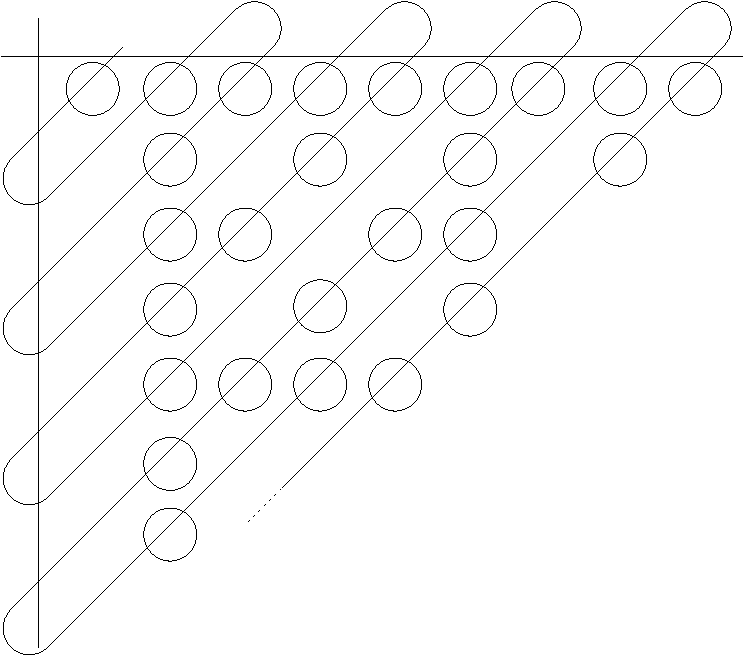
\includegraphics{./Cantor_snake.pdf}%
\end{picture}%
\setlength{\unitlength}{3947sp}%
%
\begingroup\makeatletter\ifx\SetFigFont\undefined%
\gdef\SetFigFont#1#2#3#4#5{%
  \reset@font\fontsize{#1}{#2pt}%
  \fontfamily{#3}\fontseries{#4}\fontshape{#5}%
  \selectfont}%
\fi\endgroup%
\begin{picture}(5949,5243)(1189,-5157)
\put(1801,-286){\makebox(0,0)[lb]{\smash{{\SetFigFont{12}{14.4}{\rmdefault}{\mddefault}{\updefault}{\color[rgb]{0,0,0}0}%
}}}}
\put(2401,-286){\makebox(0,0)[lb]{\smash{{\SetFigFont{12}{14.4}{\rmdefault}{\mddefault}{\updefault}{\color[rgb]{0,0,0}1}%
}}}}
\put(3001,-286){\makebox(0,0)[lb]{\smash{{\SetFigFont{12}{14.4}{\rmdefault}{\mddefault}{\updefault}{\color[rgb]{0,0,0}2}%
}}}}
\put(3601,-286){\makebox(0,0)[lb]{\smash{{\SetFigFont{12}{14.4}{\rmdefault}{\mddefault}{\updefault}{\color[rgb]{0,0,0}3}%
}}}}
\put(4201,-286){\makebox(0,0)[lb]{\smash{{\SetFigFont{12}{14.4}{\rmdefault}{\mddefault}{\updefault}{\color[rgb]{0,0,0}4}%
}}}}
\put(4801,-286){\makebox(0,0)[lb]{\smash{{\SetFigFont{12}{14.4}{\rmdefault}{\mddefault}{\updefault}{\color[rgb]{0,0,0}5}%
}}}}
\put(5401,-286){\makebox(0,0)[lb]{\smash{{\SetFigFont{12}{14.4}{\rmdefault}{\mddefault}{\updefault}{\color[rgb]{0,0,0}6}%
}}}}
\put(6001,-286){\makebox(0,0)[lb]{\smash{{\SetFigFont{12}{14.4}{\rmdefault}{\mddefault}{\updefault}{\color[rgb]{0,0,0}7}%
}}}}
\put(6601,-286){\makebox(0,0)[lb]{\smash{{\SetFigFont{12}{14.4}{\rmdefault}{\mddefault}{\updefault}{\color[rgb]{0,0,0}8}%
}}}}
\put(1351,-661){\makebox(0,0)[lb]{\smash{{\SetFigFont{12}{14.4}{\rmdefault}{\mddefault}{\updefault}{\color[rgb]{0,0,0}1}%
}}}}
\put(1351,-1261){\makebox(0,0)[lb]{\smash{{\SetFigFont{12}{14.4}{\rmdefault}{\mddefault}{\updefault}{\color[rgb]{0,0,0}2}%
}}}}
\put(1351,-1861){\makebox(0,0)[lb]{\smash{{\SetFigFont{12}{14.4}{\rmdefault}{\mddefault}{\updefault}{\color[rgb]{0,0,0}3}%
}}}}
\put(1351,-2461){\makebox(0,0)[lb]{\smash{{\SetFigFont{12}{14.4}{\rmdefault}{\mddefault}{\updefault}{\color[rgb]{0,0,0}4}%
}}}}
\put(1351,-3061){\makebox(0,0)[lb]{\smash{{\SetFigFont{12}{14.4}{\rmdefault}{\mddefault}{\updefault}{\color[rgb]{0,0,0}5}%
}}}}
\put(1351,-3661){\makebox(0,0)[lb]{\smash{{\SetFigFont{12}{14.4}{\rmdefault}{\mddefault}{\updefault}{\color[rgb]{0,0,0}6}%
}}}}
\put(1351,-4261){\makebox(0,0)[lb]{\smash{{\SetFigFont{12}{14.4}{\rmdefault}{\mddefault}{\updefault}{\color[rgb]{0,0,0}7}%
}}}}
\put(1351,-4861){\makebox(0,0)[lb]{\smash{{\SetFigFont{12}{14.4}{\rmdefault}{\mddefault}{\updefault}{\color[rgb]{0,0,0}8}%
}}}}
\put(1801,-661){\makebox(0,0)[lb]{\smash{{\SetFigFont{12}{14.4}{\rmdefault}{\mddefault}{\updefault}{\color[rgb]{0,0,0}0/1}%
}}}}
\put(2401,-661){\makebox(0,0)[lb]{\smash{{\SetFigFont{12}{14.4}{\rmdefault}{\mddefault}{\updefault}{\color[rgb]{0,0,0}1/1}%
}}}}
\put(3001,-661){\makebox(0,0)[lb]{\smash{{\SetFigFont{12}{14.4}{\rmdefault}{\mddefault}{\updefault}{\color[rgb]{0,0,0}2/1}%
}}}}
\put(3601,-661){\makebox(0,0)[lb]{\smash{{\SetFigFont{12}{14.4}{\rmdefault}{\mddefault}{\updefault}{\color[rgb]{0,0,0}3/1}%
}}}}
\put(4201,-661){\makebox(0,0)[lb]{\smash{{\SetFigFont{12}{14.4}{\rmdefault}{\mddefault}{\updefault}{\color[rgb]{0,0,0}4/1}%
}}}}
\put(4801,-661){\makebox(0,0)[lb]{\smash{{\SetFigFont{12}{14.4}{\rmdefault}{\mddefault}{\updefault}{\color[rgb]{0,0,0}5/1}%
}}}}
\put(5401,-661){\makebox(0,0)[lb]{\smash{{\SetFigFont{12}{14.4}{\rmdefault}{\mddefault}{\updefault}{\color[rgb]{0,0,0}6/1}%
}}}}
\put(6001,-661){\makebox(0,0)[lb]{\smash{{\SetFigFont{12}{14.4}{\rmdefault}{\mddefault}{\updefault}{\color[rgb]{0,0,0}7/1}%
}}}}
\put(6601,-661){\makebox(0,0)[lb]{\smash{{\SetFigFont{12}{14.4}{\rmdefault}{\mddefault}{\updefault}{\color[rgb]{0,0,0}8/1}%
}}}}
\put(1801,-1261){\makebox(0,0)[lb]{\smash{{\SetFigFont{12}{14.4}{\rmdefault}{\mddefault}{\updefault}{\color[rgb]{0,0,0}0/2}%
}}}}
\put(2401,-1261){\makebox(0,0)[lb]{\smash{{\SetFigFont{12}{14.4}{\rmdefault}{\mddefault}{\updefault}{\color[rgb]{0,0,0}1/2}%
}}}}
\put(3001,-1261){\makebox(0,0)[lb]{\smash{{\SetFigFont{12}{14.4}{\rmdefault}{\mddefault}{\updefault}{\color[rgb]{0,0,0}2/2}%
}}}}
\put(3601,-1261){\makebox(0,0)[lb]{\smash{{\SetFigFont{12}{14.4}{\rmdefault}{\mddefault}{\updefault}{\color[rgb]{0,0,0}3/2}%
}}}}
\put(4201,-1261){\makebox(0,0)[lb]{\smash{{\SetFigFont{12}{14.4}{\rmdefault}{\mddefault}{\updefault}{\color[rgb]{0,0,0}4/2}%
}}}}
\put(4801,-1261){\makebox(0,0)[lb]{\smash{{\SetFigFont{12}{14.4}{\rmdefault}{\mddefault}{\updefault}{\color[rgb]{0,0,0}5/2}%
}}}}
\put(5401,-1261){\makebox(0,0)[lb]{\smash{{\SetFigFont{12}{14.4}{\rmdefault}{\mddefault}{\updefault}{\color[rgb]{0,0,0}6/2}%
}}}}
\put(6001,-1261){\makebox(0,0)[lb]{\smash{{\SetFigFont{12}{14.4}{\rmdefault}{\mddefault}{\updefault}{\color[rgb]{0,0,0}7/2}%
}}}}
\put(6601,-1261){\makebox(0,0)[lb]{\smash{{\SetFigFont{12}{14.4}{\rmdefault}{\mddefault}{\updefault}{\color[rgb]{0,0,0}8/2}%
}}}}
\put(1801,-1861){\makebox(0,0)[lb]{\smash{{\SetFigFont{12}{14.4}{\rmdefault}{\mddefault}{\updefault}{\color[rgb]{0,0,0}0/3}%
}}}}
\put(2401,-1861){\makebox(0,0)[lb]{\smash{{\SetFigFont{12}{14.4}{\rmdefault}{\mddefault}{\updefault}{\color[rgb]{0,0,0}1/3}%
}}}}
\put(3001,-1861){\makebox(0,0)[lb]{\smash{{\SetFigFont{12}{14.4}{\rmdefault}{\mddefault}{\updefault}{\color[rgb]{0,0,0}2/3}%
}}}}
\put(3601,-1861){\makebox(0,0)[lb]{\smash{{\SetFigFont{12}{14.4}{\rmdefault}{\mddefault}{\updefault}{\color[rgb]{0,0,0}3/3}%
}}}}
\put(4201,-1861){\makebox(0,0)[lb]{\smash{{\SetFigFont{12}{14.4}{\rmdefault}{\mddefault}{\updefault}{\color[rgb]{0,0,0}4/3}%
}}}}
\put(4801,-1861){\makebox(0,0)[lb]{\smash{{\SetFigFont{12}{14.4}{\rmdefault}{\mddefault}{\updefault}{\color[rgb]{0,0,0}5/3}%
}}}}
\put(5401,-1861){\makebox(0,0)[lb]{\smash{{\SetFigFont{12}{14.4}{\rmdefault}{\mddefault}{\updefault}{\color[rgb]{0,0,0}6/3}%
}}}}
\put(6001,-1861){\makebox(0,0)[lb]{\smash{{\SetFigFont{12}{14.4}{\rmdefault}{\mddefault}{\updefault}{\color[rgb]{0,0,0}7/3}%
}}}}
\put(6601,-1861){\makebox(0,0)[lb]{\smash{{\SetFigFont{12}{14.4}{\rmdefault}{\mddefault}{\updefault}{\color[rgb]{0,0,0}8/3}%
}}}}
\put(1801,-2461){\makebox(0,0)[lb]{\smash{{\SetFigFont{12}{14.4}{\rmdefault}{\mddefault}{\updefault}{\color[rgb]{0,0,0}0/4}%
}}}}
\put(2401,-2461){\makebox(0,0)[lb]{\smash{{\SetFigFont{12}{14.4}{\rmdefault}{\mddefault}{\updefault}{\color[rgb]{0,0,0}1/4}%
}}}}
\put(3001,-2461){\makebox(0,0)[lb]{\smash{{\SetFigFont{12}{14.4}{\rmdefault}{\mddefault}{\updefault}{\color[rgb]{0,0,0}2/4}%
}}}}
\put(3601,-2461){\makebox(0,0)[lb]{\smash{{\SetFigFont{12}{14.4}{\rmdefault}{\mddefault}{\updefault}{\color[rgb]{0,0,0}3/4}%
}}}}
\put(4201,-2461){\makebox(0,0)[lb]{\smash{{\SetFigFont{12}{14.4}{\rmdefault}{\mddefault}{\updefault}{\color[rgb]{0,0,0}4/4}%
}}}}
\put(4801,-2461){\makebox(0,0)[lb]{\smash{{\SetFigFont{12}{14.4}{\rmdefault}{\mddefault}{\updefault}{\color[rgb]{0,0,0}5/4}%
}}}}
\put(5401,-2461){\makebox(0,0)[lb]{\smash{{\SetFigFont{12}{14.4}{\rmdefault}{\mddefault}{\updefault}{\color[rgb]{0,0,0}6/4}%
}}}}
\put(6001,-2461){\makebox(0,0)[lb]{\smash{{\SetFigFont{12}{14.4}{\rmdefault}{\mddefault}{\updefault}{\color[rgb]{0,0,0}7/4}%
}}}}
\put(6601,-2461){\makebox(0,0)[lb]{\smash{{\SetFigFont{12}{14.4}{\rmdefault}{\mddefault}{\updefault}{\color[rgb]{0,0,0}8/4}%
}}}}
\put(1801,-3061){\makebox(0,0)[lb]{\smash{{\SetFigFont{12}{14.4}{\rmdefault}{\mddefault}{\updefault}{\color[rgb]{0,0,0}0/5}%
}}}}
\put(2401,-3061){\makebox(0,0)[lb]{\smash{{\SetFigFont{12}{14.4}{\rmdefault}{\mddefault}{\updefault}{\color[rgb]{0,0,0}1/5}%
}}}}
\put(3001,-3061){\makebox(0,0)[lb]{\smash{{\SetFigFont{12}{14.4}{\rmdefault}{\mddefault}{\updefault}{\color[rgb]{0,0,0}2/5}%
}}}}
\put(3601,-3061){\makebox(0,0)[lb]{\smash{{\SetFigFont{12}{14.4}{\rmdefault}{\mddefault}{\updefault}{\color[rgb]{0,0,0}3/5}%
}}}}
\put(4201,-3061){\makebox(0,0)[lb]{\smash{{\SetFigFont{12}{14.4}{\rmdefault}{\mddefault}{\updefault}{\color[rgb]{0,0,0}4/5}%
}}}}
\put(4801,-3061){\makebox(0,0)[lb]{\smash{{\SetFigFont{12}{14.4}{\rmdefault}{\mddefault}{\updefault}{\color[rgb]{0,0,0}5/5}%
}}}}
\put(5401,-3061){\makebox(0,0)[lb]{\smash{{\SetFigFont{12}{14.4}{\rmdefault}{\mddefault}{\updefault}{\color[rgb]{0,0,0}6/5}%
}}}}
\put(6001,-3061){\makebox(0,0)[lb]{\smash{{\SetFigFont{12}{14.4}{\rmdefault}{\mddefault}{\updefault}{\color[rgb]{0,0,0}7/5}%
}}}}
\put(6601,-3061){\makebox(0,0)[lb]{\smash{{\SetFigFont{12}{14.4}{\rmdefault}{\mddefault}{\updefault}{\color[rgb]{0,0,0}8/5}%
}}}}
\put(1801,-3661){\makebox(0,0)[lb]{\smash{{\SetFigFont{12}{14.4}{\rmdefault}{\mddefault}{\updefault}{\color[rgb]{0,0,0}0/6}%
}}}}
\put(2401,-3661){\makebox(0,0)[lb]{\smash{{\SetFigFont{12}{14.4}{\rmdefault}{\mddefault}{\updefault}{\color[rgb]{0,0,0}1/6}%
}}}}
\put(3001,-3661){\makebox(0,0)[lb]{\smash{{\SetFigFont{12}{14.4}{\rmdefault}{\mddefault}{\updefault}{\color[rgb]{0,0,0}2/6}%
}}}}
\put(3601,-3661){\makebox(0,0)[lb]{\smash{{\SetFigFont{12}{14.4}{\rmdefault}{\mddefault}{\updefault}{\color[rgb]{0,0,0}3/6}%
}}}}
\put(4201,-3661){\makebox(0,0)[lb]{\smash{{\SetFigFont{12}{14.4}{\rmdefault}{\mddefault}{\updefault}{\color[rgb]{0,0,0}4/6}%
}}}}
\put(4801,-3661){\makebox(0,0)[lb]{\smash{{\SetFigFont{12}{14.4}{\rmdefault}{\mddefault}{\updefault}{\color[rgb]{0,0,0}5/6}%
}}}}
\put(5401,-3661){\makebox(0,0)[lb]{\smash{{\SetFigFont{12}{14.4}{\rmdefault}{\mddefault}{\updefault}{\color[rgb]{0,0,0}6/6}%
}}}}
\put(6001,-3661){\makebox(0,0)[lb]{\smash{{\SetFigFont{12}{14.4}{\rmdefault}{\mddefault}{\updefault}{\color[rgb]{0,0,0}7/6}%
}}}}
\put(6601,-3661){\makebox(0,0)[lb]{\smash{{\SetFigFont{12}{14.4}{\rmdefault}{\mddefault}{\updefault}{\color[rgb]{0,0,0}8/6}%
}}}}
\put(1801,-4261){\makebox(0,0)[lb]{\smash{{\SetFigFont{12}{14.4}{\rmdefault}{\mddefault}{\updefault}{\color[rgb]{0,0,0}0/7}%
}}}}
\put(2401,-4261){\makebox(0,0)[lb]{\smash{{\SetFigFont{12}{14.4}{\rmdefault}{\mddefault}{\updefault}{\color[rgb]{0,0,0}1/7}%
}}}}
\put(3001,-4261){\makebox(0,0)[lb]{\smash{{\SetFigFont{12}{14.4}{\rmdefault}{\mddefault}{\updefault}{\color[rgb]{0,0,0}2/7}%
}}}}
\put(3601,-4261){\makebox(0,0)[lb]{\smash{{\SetFigFont{12}{14.4}{\rmdefault}{\mddefault}{\updefault}{\color[rgb]{0,0,0}3/7}%
}}}}
\put(4201,-4261){\makebox(0,0)[lb]{\smash{{\SetFigFont{12}{14.4}{\rmdefault}{\mddefault}{\updefault}{\color[rgb]{0,0,0}4/7}%
}}}}
\put(4801,-4261){\makebox(0,0)[lb]{\smash{{\SetFigFont{12}{14.4}{\rmdefault}{\mddefault}{\updefault}{\color[rgb]{0,0,0}5/7}%
}}}}
\put(5401,-4261){\makebox(0,0)[lb]{\smash{{\SetFigFont{12}{14.4}{\rmdefault}{\mddefault}{\updefault}{\color[rgb]{0,0,0}6/7}%
}}}}
\put(6001,-4261){\makebox(0,0)[lb]{\smash{{\SetFigFont{12}{14.4}{\rmdefault}{\mddefault}{\updefault}{\color[rgb]{0,0,0}7/7}%
}}}}
\put(6601,-4261){\makebox(0,0)[lb]{\smash{{\SetFigFont{12}{14.4}{\rmdefault}{\mddefault}{\updefault}{\color[rgb]{0,0,0}8/7}%
}}}}
\put(1801,-4861){\makebox(0,0)[lb]{\smash{{\SetFigFont{12}{14.4}{\rmdefault}{\mddefault}{\updefault}{\color[rgb]{0,0,0}0/8}%
}}}}
\put(2401,-4861){\makebox(0,0)[lb]{\smash{{\SetFigFont{12}{14.4}{\rmdefault}{\mddefault}{\updefault}{\color[rgb]{0,0,0}1/8}%
}}}}
\put(3001,-4861){\makebox(0,0)[lb]{\smash{{\SetFigFont{12}{14.4}{\rmdefault}{\mddefault}{\updefault}{\color[rgb]{0,0,0}2/8}%
}}}}
\put(3601,-4861){\makebox(0,0)[lb]{\smash{{\SetFigFont{12}{14.4}{\rmdefault}{\mddefault}{\updefault}{\color[rgb]{0,0,0}3/8}%
}}}}
\put(4201,-4861){\makebox(0,0)[lb]{\smash{{\SetFigFont{12}{14.4}{\rmdefault}{\mddefault}{\updefault}{\color[rgb]{0,0,0}4/8}%
}}}}
\put(4801,-4861){\makebox(0,0)[lb]{\smash{{\SetFigFont{12}{14.4}{\rmdefault}{\mddefault}{\updefault}{\color[rgb]{0,0,0}5/8}%
}}}}
\put(5401,-4861){\makebox(0,0)[lb]{\smash{{\SetFigFont{12}{14.4}{\rmdefault}{\mddefault}{\updefault}{\color[rgb]{0,0,0}6/8}%
}}}}
\put(6001,-4861){\makebox(0,0)[lb]{\smash{{\SetFigFont{12}{14.4}{\rmdefault}{\mddefault}{\updefault}{\color[rgb]{0,0,0}7/8}%
}}}}
\put(6601,-4861){\makebox(0,0)[lb]{\smash{{\SetFigFont{12}{14.4}{\rmdefault}{\mddefault}{\updefault}{\color[rgb]{0,0,0}8/8}%
}}}}
\end{picture}%

\end{center}

\workbookpagebreak

Effectively this gives us a function $f$ which produces the rational number 
that would be found in a given position in this list.  For example 
$f(1) = 0/1, f(2) = 1/1$ and $f(5) = 1/3$.  

What is $f(26)$?  What is $f(30)$?  What is $f^{-1}(3/4)$? What is $f^{-1}(6/7)$?


  
\wbvfill

\workbookpagebreak
 
\end{enumerate}


%% Emacs customization
%% 
%% Local Variables: ***
%% TeX-master: "GIAM-hw.tex" ***
%% comment-column:0 ***
%% comment-start: "%% "  ***
%% comment-end:"***" ***
%% End: ***


\newpage

\section{Special functions}
\label{sec:special_functions}

%restrictions

There are a great many functions that fail the horizontal line test
which we nevertheless seem to have inverse functions for.  For example,
$x^2$ fails HLT but $\sqrt{x}$ is a pretty reasonable inverse for it --
one just needs to be careful about the ``plus or minus'' issue.  Also,
$\sin{x}$ fails HLT pretty badly; any horizontal line $y=c$ with 
$-1 \leq c \leq 1$ will hit $\sin{x}$ infinitely many times.  But look!
Right here on my calculator is a button labeled ``$\sin^{-1}$.''\footnote{It 
might be labeled ``asin'' instead.  The old-style way to refer to the inverse
of a trig. function was arc-whatever.  So the inverse of sine was arcsine,
the inverse of tangent was arctangent.}  This apparent contradiction
can be resolved using the notion of restriction.

\begin{defi}
\index{restriction, of a function}
Given a function $f$ and a subset $D$ of its domain, the
\emph{restriction of $f$ to $D$} is denoted $\restrict{f}{D}$ and

\[ \restrict{f}{D} = \{ (x,y) \suchthat \; x \in D \, \land \, (x,y) \in f \}. \]
\end{defi}

The way we typically use restriction is to eliminate any regions in
$\Dom{f}$ that cause $f$ to fail to be one-to-one.   That is, we
choose a subset $D \subseteq \Dom{f}$ so that $\restrict{f}{D}$ is an injection.
This allows us to invert the restricted version of $f$.  There can be
problems in doing this, but if we are careful about how we choose $D$,
these problems are usually resolvable.

\begin{exer}
Suppose $f$ is a function that is not one-to-one, and $D$ is a subset
of $\Dom{f}$ such that $\restrict{f}{D}$ \emph{is} one-to-one.  The restricted
function $\restrict{f}{D}$ has an inverse which we will denote by $g$.  
Note that $g$ is a function from $\Rng{\restrict{f}{D}}$ to $D$.  Which
of the following is always true:

\[ f(g(x)) = x \quad \mbox{or} \quad g(f(x)) = x ? \]
\end{exer}

Technically, when we do the process outlined above (choose a domain
$D$ so that the restriction $\restrict{f}{D}$ is invertible, and 
find that inverse)
the function we get is a \index{right inverse}\emph{right inverse} for $f$.

Let's take a closer look at the inverse sine function.  This should 
help us to really understand the ``right inverse'' concept.  

A glance at the graph of $y = \sin{x}$ will certainly convince us that 
this function is not injective, but the portion of the graph shown 
in bold below passes the horizontal line test.

\begin{center}
\begin{picture}(0,0)%
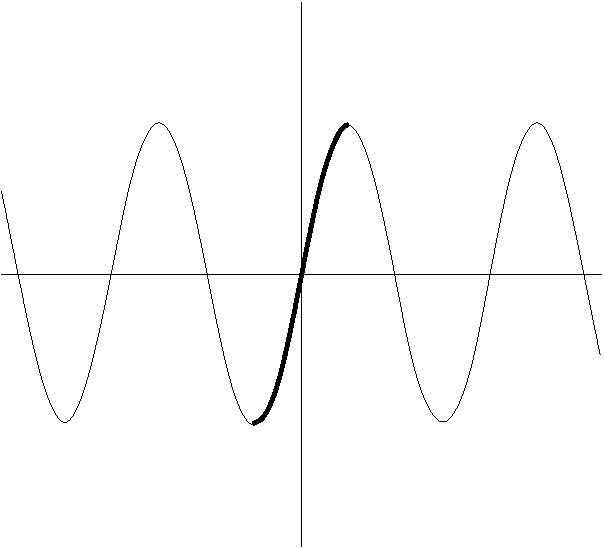
\includegraphics{figures/graph_o_sine.pdf}%
\end{picture}%
\setlength{\unitlength}{3947sp}%
%
\begingroup\makeatletter\ifx\SetFigFont\undefined%
\gdef\SetFigFont#1#2#3#4#5{%
  \reset@font\fontsize{#1}{#2pt}%
  \fontfamily{#3}\fontseries{#4}\fontshape{#5}%
  \selectfont}%
\fi\endgroup%
\begin{picture}(4827,4374)(3136,-5098)
\end{picture}%

\end{center}

If we restrict the domain of the sine function to the closed interval 
$[-\pi/2, \pi/2]$, we have an invertible function.  The inverse of this
restricted function is the function we know as $\sin^{-1}(x)$ or 
$\mbox{arcsin}(x)$.  The domain and range of $\sin^{-1}(x)$ are 
(respectively) the intervals
$[-1,1]$ and $[-\pi/2, \pi/2]$.  

Notice that if we choose a number $x$ in the range $-1 \leq x \leq 1$ and apply
the inverse sine function to it, we will get a number between $-\pi/2$ and 
$\pi/2$ -- i.e. a number we can interpret as an \emph{angle} in radian measure.
If we then proceed to calculate the sine of this angle, we will get back our
original number $x$.

On the other hand, if we choose an angle first, then take the sine of it to
get a number in $[-1,1]$ and then take the inverse sine of \emph{that},
we will only end up with the same angle we started with {\bf if} 
we chose the original angle
so that it lay in the interval $[-\pi/2, \pi/2]$.

\begin{exer}
We get a right inverse for the cosine function by restricting it to
the interval $[0,\pi]$.  What are the domain and range of $\cos^{-1}$?
\end{exer} 

The \index{winding map}\emph{winding map} is a function that goes 
from $\Reals$ to the unit circle in the $x$--$y$ plane, defined by

\[ W(t) = (\cos{t}, \sin{t}). \]

One can think of this map as literally winding the infinitely long
real line around and around the circle.   Obviously, this is not an
injection -- there are an infinite number of values of $t$ that 
get mapped to (for instance) the point $(1,0)$, $t$ can be any integer
multiple of $2\pi$.

\begin{exer}
What is the set $W^{-1}(\{(0,1)\})$ ?
\end{exer}

If we restrict $W$ to the half-open interval $[0, 2\pi)$ the restricted
function $\restrict{W}{[0, 2\pi)}$ is an injection.  The inverse function is 
not easy to write down, but it is possible to express (in terms 
of the inverse functions of sine and cosine) if we consider the 
four cases determined by what quadrant a point on the unit circle 
may lie in.

\begin{exer}
Suppose $(x,y)$ represents a point on the unit circle.  If $(x,y)$ happens
to lie on one of the coordinate axes we have 

\begin{gather*}
W^{-1}((1,0)) = 0\\
W^{-1}((0,1)) = \pi/2\\
W^{-1}((-1,0)) = \pi\\
W^{-1}((0,-1)) = 3\pi/2.\\
\end{gather*}

If neither $x$ nor $y$ is zero, there are four cases to consider.
Write an expression for $W^{-1}((x,y))$ using the cases 
(i) $x>0 \, \land \, y>0$, 
(ii) $x<0 \, \land \, y>0$, 
(iii) $x<0 \, \land \, y<0$ and  
(iv) $x>0 \, \land \, y<0$. 

\end{exer}

This last example that we have done (the winding map) was unusual in that
the outputs were ordered pairs.  In thinking of this map as a relation
(that is, as a set of ordered pairs) we have an ordered pair in which 
the second element is an ordered pair!  Just for fun, here is another 
way of expressing the winding map:

\[ W = \{ (t, (\cos{t}, \sin{t})) \suchthat \, t \in \Reals \} \]

When dealing with very complicated expressions involving ordered
pairs, or more generally, ordered $n$-tuples, it is useful to 
have a way to refer succinctly to the pieces of a tuple.

Let's start by considering the set $P = \Reals \times \Reals$ --- i.e. 
$P$ is the $x$--$y$ plane.  There are two functions, whose domain is $P$
that ``pick out'' the $x$, and/or $y$ coordinate.  These functions are
called $\pi_1$ and $\pi_2$, $\pi_1$ is the projection onto the first
coordinate and $\pi_2$ is the projection onto the second coordinate.\footnote{%
Don't think of the usual $\pi \approx 3.14159$ when looking at $\pi_1$ and %
$\pi_2$.  These functions are named as they are because $\pi$ is the Greek %
letter corresponding to `p' which stands for ``projection.''}

\begin{defi}
The function $\pi_1: \Reals \times \Reals \longrightarrow \Reals$ known
as \index{projection}\emph{projection onto the first coordinate} is
defined by

\[ \pi_1((x,y)) = x. \]
 
\end{defi}

The definition of $\pi_2$ is entirely analogous.  

You should note that these projection functions are \emph{very} bad 
as far as being one-to-one is concerned.  For instance, the preimage
of $1$ under the map $\pi_1$ consists of all the points on the vertical line
$x=1$.  That's a lot of preimages!  These guys are so far from being 
one-to-one that it seems impossible to think of an appropriate restriction
that would become invertible.  Nevertheless, there is a function that 
provides a right inverse for both $\pi_1$ and $\pi_2$.  Now, these projection
maps go from $\Reals \times \Reals$ to $\Reals$ so an inverse needs to be
a map from $\Reals$ to $\Reals \times \Reals$.  What is a reasonable way to
produce a \emph{pair} of real numbers if we have a single real number in hand?
There are actually many ways one could proceed, but one reasonable choice is
to create a pair where the input number appears in both coordinates.  This
is the so-called \index{diagonal map}\emph{diagonal map}, 
$d:\Reals \times \Reals \longrightarrow \Reals$, defined by $d(a) = (a,a)$.

\begin{exer}
Which of the following is always true,

\[ d(\pi_1((x,y)) = (x,y) \quad \mbox{or} \quad \pi_1(d(x)) = x? \] 
\end{exer}


There are a few other functions that it will be convenient to 
introduce at this stage.  All of them are aspects of the 
characteristic function of a subset, so we'll start with that.

Whenever we have a subset/superset relationship, $S \subseteq D$,  
it is possible to define a function whose codomain is $\{0,1\}$
which performs a very useful task -- if an input $x$ is in the 
set $S$ the function will indicate this by returning 1, otherwise
it will return 0.   The function which has this behavior is known 
as $1_S$, and is called the \index{characteristic function}
\emph{characteristic function of the subset $S$} (There are those
who use the term \index{indicator function}\emph{indicator function of $S$}
for $1_S$.)  By definition,
$D$ is the domain of this function.  

\begin{gather*}
1_S: D \longrightarrow \{0,1\} \\
1_S(x) = \left\{ \begin{array}{cl} 1 & \mbox{if} \, x \in S \\ 0 & \mbox{otherwise} \end{array} \right.  
\end{gather*}

\begin{exer}
If you have the characteristic function of a subset $S$, how can you
create the characteristic function of its complement, $\overline{S}$.
\end{exer}

A characteristic function may be thought of as an embodiment of a
membership criterion.  The logical open sentence ``$x \in S$'' being true
is the same thing as the equation ``$1_S(x) = 1$.''   There is a notation,
growing in popularity, that does the same thing for an arbitrary open sentence.
The \index{Iverson bracket}\emph{Iverson bracket} notation uses the 
shorthand $[ P(x) ]$ to represent a function that sends any $x$ that makes
$P(x)$ true to 1, and any inputs that make $P(x)$ false will get sent to 0.

\[ [ P(x) ] = \left\{ \begin{array}{cl} 1 & \mbox{if} \, P(x) \\ 0 & \mbox{otherwise} \end{array} \right.  \]
 
The Iverson brackets can be particularly useful in expressing and simplifying
sums.  For example, we can write $\sum_{i=1}^{24} [2 \divides i]$ to
find the number of even natural numbers less than 25.  Similarly, we can write
$\sum_{i=1}^{24} [3 \divides i]$ to find the number of natural numbers less than 
25 that are divisible by 3.  

\begin{exer}
What does the following formula count?

\[ \sum_{i=1}^{24} [2 \divides i] + [3 \divides i] - [6 \divides i] \]

\end{exer} 

There is a much more venerable notation known as the \index{Kronecker delta}
\emph{Kronecker delta} that can be thought of as a special case of the 
idea inherent in Iverson brackets.  We write $\delta_{ij}$ as a shorthand
for a function that takes two inputs, $\delta(i,j)$ is 1 if and only if
$i$ and $j$ are equal.

\[ \delta_{ij} =  \left\{ \begin{array}{cl} 1 & \mbox{if} \; i=j \\ 0 & \mbox{otherwise} \end{array} \right.  \]

The corresponding Iverson bracket would simply be $[i=j]$.

We'll end this section with a function that will be especially important
in Chapter~\ref{ch:card}.   If we have an arbitrary subset of the natural
numbers, we can associate it with an infinite string of 0's and 1's.  By
sticking a decimal point in front of such a thing, we get binary notation
for a real number in the interval $[0,1]$.  There is a subtle problem that 
we'll deal with when we study this function in more detail in Chapter~\ref{ch:card} --- some real numbers can be expressed in two different ways in base 2.
For example, $1/2$ can either be written as $.1$ or as $.0\overline{1}$ (where,
as usual, the overline indicates a pattern that repeats forever).  
For the moment, we are talking about 
defining a function $\phi$ whose domain is ${\mathcal P}(\Naturals)$ and 
whose codomain is the set of all infinite binary strings. 
Let us denote these binary expansions by
$.b_1b_2b_3b_4\ldots$.  Suppose $A$ is a subset of $\Naturals$,
then the binary expansion associated with $A$ will be
determined by $b_i = 1_A(i)$.  (Alternatively, we can use the Iverson 
bracket notation: $b_i = [i \in A]$.)   

The function $\phi$ defined in the last paragraph turns out to be a 
bijection -- given a subset we get a unique binary expansion, and given 
binary expansion we get (using $\phi^{-1}$) a unique subset  of 
$\Naturals$.

A few examples will
probably help to clarify this function's workings.  Consider 
the set $\{1,2,3\} \subseteq \Naturals$, the binary expansion that this
corresponds to will have 1's in the first three positions after the 
decimal -- $\phi(\{1,2,3\}) = .111$ this is the number written .875
in decimal.  The infinite repeating binary number $.\overline{01}$ 
is the base-2 representation of $1/3$, it is easy to see that
$.\overline{01}$ is the image of the set of odd naturals, $\{1,3,5,\ldots\}$.

\begin{exer}
Find the binary representation for the real number which is the image of
the set of even numbers under $\phi$.  
\end{exer}

\begin{exer}
Find the binary representation for the real number which is the image of
the set of triangular numbers under $\phi$.  (Recall that the triangular
numbers are $T = \{1,3,6,10,15, \ldots \}$.)
\end{exer}

\newpage

\noindent{\large \bf Exercises --- \thesection\ }

\begin{enumerate}

\item The $n$-th triangular number, denoted $T(n)$, is given by the formula
$T(n) = (n^2 + n)/2$. If we regard this formula as a function from $\Reals$ to
$\Reals$, it fails the horizontal line test and so it is not invertible. Find a
suitable restriction so that T is invertible.

\wbvfill

\item The usual algebraic procedure for inverting $T(x) = (x^2+x)/2$ fails. Use
your knowledge of the geometry of functions and their inverses to find
a formula for the inverse. (Hint: it may be instructive to first invert
the simpler formula $S(x) = x^2/2$ --- this will get you the right vertical
scaling factor.)

\wbvfill

\item What is $\pi_2(W(t))$?  

\wbvfill

\item Find a right inverse for $f(x) = |x|$.

\wbvfill

\workbookpagebreak

\item In three-dimensional space we have projection functions that go onto
the three coordinate axes ($\pi_1$, $\pi_2$ and $\pi_3$) and we also have
projections onto coordinate planes.  For example,
$\pi_{12}: \Reals \times \Reals \times \Reals \longrightarrow \Reals \times \Reals$, defined by

\[ \pi_{12}((x,y,z)) = (x,y) \]

\noindent is the projection onto the $x$--$y$ coordinate plane.

The triple of functions  $(\cos{t}, \sin{t}, t)$ is a parametric
expression for a helix.  Let 
$H = \{ (\cos{t}, \sin{t}, t) \suchthat t \in \Reals \}$ be the set of all
points on the helix.  What is the set $\pi_{12}(H)$ ?  What are the
sets $\pi_{13}(H)$ and $\pi_{23}(H)$?

\wbvfill

\workbookpagebreak

\item Consider the set $\{1, 2, 3, \ldots, 10\}$.  Express the characteristic
function of the subset $S = \{1, 2, 3 \}$ as a set of ordered pairs.

\wbvfill

%\workbookpagebreak

\item If $S$ and $T$ are subsets of a set $D$, what is the product of
their characteristic functions $1_S \cdot 1_T$ ?

\wbvfill

%\workbookpagebreak

\item Evaluate the sum

\[ \sum_{i=1}^{10} \frac{1}{i} \cdot [ i \; \mbox{is prime} ]. \]

\wbvfill

\workbookpagebreak
\end{enumerate}

%% Emacs customization
%% 
%% Local Variables: ***
%% TeX-master: "GIAM-hw.tex" ***
%% comment-column:0 ***
%% comment-start: "%% "  ***
%% comment-end:"***" ***
%% End: ***


%% Emacs customization
%% 
%% Local Variables: ***
%% TeX-master: "GIAM.tex" ***
%% comment-column:0 ***
%% comment-start: "%% "  ***
%% comment-end:"***" ***
%% End: ***
